% ---------------------------------------------------------------------------
% Author guideline and sample document for EG publication using LaTeX2e input
% D.Fellner, v1.13, Jul 31, 2008

\documentclass{egpubl}
\usepackage{eg2015}

% --- for  Annual CONFERENCE
\ConferenceSubmission   % uncomment for Conference submission
%\ConferencePaper        % uncomment for (final) Conference Paper
% \STAR                   % uncomment for STAR contribution
% \Tutorial               % uncomment for Tutorial contribution
% \ShortPresentation      % uncomment for (final) Short Conference Presentation
% \Areas                  % uncomment for Areas contribution
% \MedicalPrize           % uncomment for Medical Prize contribution
% \Education              % uncomment for Education contribution
%
% --- for  CGF Journal
% \JournalSubmission    % uncomment for submission to Computer Graphics Forum
% \JournalPaper         % uncomment for final version of Journal Paper
%
% --- for  CGF Journal: special issue
% \SpecialIssueSubmission    % uncomment for submission to Computer Graphics Forum, special issue
% \SpecialIssuePaper         % uncomment for final version of Journal Paper, special issue
%
% --- for  EG Workshop Proceedings
% \WsSubmission    % uncomment for submission to EG Workshop
% \WsPaper         % uncomment for final version of EG Workshop contribution
%
 \electronicVersion % can be used both for the printed and electronic version

% !! *please* don't change anything above
% !! unless you REALLY know what you are doing
% ------------------------------------------------------------------------

% for including postscript figures
% mind: package option 'draft' will replace PS figure by a filname within a frame
\ifpdf \usepackage[pdftex]{graphicx} \pdfcompresslevel=9
\else \usepackage[dvips]{graphicx} \fi


\PrintedOrElectronic

% prepare for electronic version of your document
% prepare for electronic version of your document
\usepackage{t1enc,dfadobe}
\usepackage{egweblnk}
\usepackage{cite}
\usepackage{epstopdf}
\usepackage{float}
\usepackage{verbatim}
\usepackage{subfigure}
\usepackage{amsmath}
\usepackage{multicol}
\usepackage{caption}
\usepackage{fontenc}
\usepackage{csquotes}
\usepackage{array}
\usepackage{graphicx}
% For backwards compatibility to old LaTeX type font selection.
% Uncomment if your document adheres to LaTeX2e recommendations.
% \let\rm=\rmfamily    \let\sf=\sffamily    \let\tt=\ttfamily
% \let\it=\itshape     \let\sl=\slshape     \let\sc=\scshape
% \let\bf=\bfseries

% end of prologue

% ------------------------------------------------------------------------

% if the Editors-in-Chief have given you the data, you may uncomment
% the following five lines and insert it here
%
% \volume{27}   % the volume in which the issue will be published;
% \issue{1}     % the issue number of the publication
% \pStartPage{1}      % set starting page


%-------------------------------------------------------------------------

% For backwards compatibility to old LaTeX type font selection.
% Uncomment if your document adheres to LaTeX2e recommendations.
% \let\rm=\rmfamily    \let\sf=\sffamily    \let\tt=\ttfamily
% \let\it=\itshape     \let\sl=\slshape     \let\sc=\scshape
% \let\bf=\bfseries

% end of prologue

%--------------------------------------------------------------
%--------------------------------------------------------------
\title[SAR: Stroke Authorship Recognition]%
      {SAR: Stroke Authorship Recognition}

% for anonymous conference submission please enter your SUBMISSION ID
% instead of the author's name (and leave the affiliation blank) !!
\author[paper1004]
     {paper1004}

% ------------------------------------------------------------------------

% if the Editors-in-Chief have given you the data, you may uncomment
% the following five lines and insert it here
%
% \volume{27}   % the volume in which the issue will be published;
% \issue{1}     % the issue number of the publication
% \pStartPage{1}      % set starting page


%-------------------------------------------------------------------------
\begin{document}


\teaser{
\centering
\includegraphics[width = 1.01\textwidth]{images/fullPipeline2.png}
\vspace{-5mm}\caption {The SAR pipeline: 1. compile sketches from different artists; 2. extract strokes and split them into segments; 3. characterize each stroke segment mathematically 4. represent each sketch as a distribution of feature frequency; 5. train a machine to recognize authorship based on 4.}%\vspace{-2mm}
\label{pipeline}}

\maketitle

\begin{abstract}
Are simple strokes unique to the artist or designer who renders them? If so, can this idea be used to identify authorship or to classify artistic drawings? Also, could training methods be devised to develop particular styles? To answer these questions, we propose the Stroke Authorship Recognition (SAR) approach, a novel method that distinguishes the authorship of 2D digitized drawings. SAR converts a drawing into a histogram of stroke attributes that is discriminative of authorship. We provide extensive classification experiments on a large variety of datasets, which validate SAR's ability to distinguish unique authorship of artists and designers. We also demonstrate the usefulness of SAR in several applications including the detection of  fraudulent sketches, the training and monitoring of artists in learning a particular new style, and the first quantitative way to measure the quality of automatic sketch synthesis tools.\vspace{-1mm}
\end{abstract}
%-------------------------------------------------------------------------
\vspace{-5mm}
\section{Introduction}
\vspace{-2mm}
Research in voice and face recognition have well-developed methods to recognize and distinguish individuals based on data cues ~\cite{tolba2006face}. Similarly, we investigate whether individuals (specifically artists) are distinguishable by the way they draw, and if so, the extent to which this uniqueness can identify their drawings, to help train them, or to detect sketch fraud. To our knowledge, this work is the first on authorship recognition from drawings. Our new method, called sketch authorship recognition, or SAR assumes that an artist's style can be recognized by the frequency distribution of certain mathematical descriptors, which are deduced from basic sketching strokes. A fundamental assumption is that the artist style manifests itself mathematically in the artist's basic strokes, For example, we have seen that Disney's Mickey Mouse tends to exhibit rounded strokes using many, nearly elliptic curves, whereas Looney Tunes Daffy Duck consists of a combination of straighter and tightly curved strokes. By extracting enough strokes from a digitized drawing, a characteristic histogram is created. This histogram captures an inherent style of the overall drawing.  As illustrated in Figure 1, SAR consists of five steps: (1) obtain sketches drawn, (2), extract strokes from each sketch, (3) split strokes into simple segments, (4) collect pertinent mathematical attributes of strokes into a frequency distribution, and (5) use (4) to train a machine to recognize the author.

\vspace{-1mm}
SAR is useful in a variety of applications such as fraud detection (i.e. fraudulent versus original sketches), where there is a need to examine fine-grained stroke-level features to discriminate sketches that \emph{look} similar. This problem cannot be approached using existing shape matching techniques, which are unable to detect local and fine differences. Also, these methods are heavily dependent on the content of the sketch and not its stlye. Moreover, SAR can play a major role in artistic style training and reproduction, since it can be used to quantitatively assess how the sketching style of an artist in-training is becoming similar to a desired target style throughout the training process. For example, newly recruited artists at Disney
are required to undergo a six month training procedure to familiarize themselves with the company's sketch techniques. This is done to ensure that new and already existing characters can be created with the same Disney \emph{look}. Clearly, there a need for an automated technique to examine how an artist progresses during his/her sketch style training. Other areas that can make use of SAR include handwriting verification, design patent litigation and brand marking.

%Techniques used in SAR can also be extended to handwriting verification applications, since automatic techniques that analyze handwriting authorship using detailed low-level features do not exist \B{I dont know whether we should say this. Reviewers might expect to see results}.
\vspace{-1mm}
\textbf{Contributions:} In this work, \textbf{(1)} we propose a novel method of sketch authorship recognition (SAR) based on the hypothesis that the collection of an artist's strokes in a sketch are unique to that artist and they can be used to define his/her style which can be used to detect sketch fraud. \textbf{(2)} We compile 2 new sketch datasets collected from  a number of experienced artists. These datasets are designed to expose SAR to different levels of challenges and sketch variations. They will be made publicly available, along with SAR source code, to allow for further research on this topic. \textbf{(3)} We develop two SAR-enabled sketch applications. The first provides artists in-training with immediate feedback on how close their sketching style is to a particular target style and monitors their progress throughout the training period. The other provides the first quantitative and automatic measure to evaluate the quality of automatic sketch synthesis tools.

%The paper is organized as follows. First, we survey the literature most related to SAR. Next, Section \ref{sec:SAR} presents a detailed description of SAR and its underlying modules. In Section \ref{sec:humanexps}, we present the details of the different datasets compiled in this work as well as 2 extensive user studies that validate the difficulty of the stroke authorship problem. Extensive experimental results and two sample applications of SAR are presented in Sections \ref{sec:exp} and \ref{sec:app} respectively. We conclude the paper and highlight future work in Section \ref{sec:conclusions}.


%As illustrated in Figure ~\ref{pipeline}, the proposed SAR approach consists of five major steps: obtaining sketches drawn by different artists, extracting strokes from each sketch, splitting strokes into segments that expose authorship, examining the characteristics of these segments to represent each sketch using features derived from these characteristics, and classifying authorship using this representation. To evaluate SAR, we compile 2 different sketch datasets collected from  a number of experienced artists. These datasets are designed to expose SAR to different levels of challenges and sketch variations so as to test its effectiveness in authorship recognition. These datasets, along with SAR source code, will be made publicly available to allow for further research in this field. \B{is this the contribution paragraph? usually contributions are made explicit}

%We hope that people in the community will find our databsets useful to use and research upon. Our collaborating artists who demonstrated through their work a great sketching abilities, have come from diverse artistic and sketching backgrounds as some of them are graphical designers and others are interior designer with an average sketching experience of 7 years and a maximum of 10 years.




%conducted to compare human versus computational sketch authorship recognition performance will be provided. After that, the development pipeline of SAR and the different techniques adopted will be provided. Towards the end of this paper, we share a number experimental results across different datasets that validate the use of SAR in authorship recognition.We will also present experimental results regarding different algorithmic variations we adopted and tested so that the community can use our findings and take them into consideration when conducting a research in the same field. Finally, we will demonstrate an application which is a training program that allows artists, designers and animators to test their affinity to any given artist, whose works have been incorporated into the machine learning part of the program.



\vspace{-3mm}
\section{Related Work}
\vspace{-2mm}
In this section, we survey previous work that is most related to our approach, grouped into four main categories.

%\vspace{-4mm}
\noindent\textbf{Shape Matching.} \label{subsec: shapematching}
%\vspace{-1mm}
Determining stroke authorship seems akin to shape matching, but has different requirements as further inspection is needed. Numerous methods have been developed for shape matching and classification in the past ~\cite{mokhtarian1992theory,belongie2001matching,jin2003image,berg2005shape}, as well as, recently \cite{Michel:2011:SID:1994006.1994152,ion-cviu-11}. Shape matching searches for similar shapes between two images, where one is usually considered the query image. Our system differs from shape matching in two main aspects. First, shape matching focuses on global information of contours such as zero crossings of curvature, while SAR segments the contour and studies detailed local features from each curve segment e.g. the eccentricity of a conic fit. Second, shape matching is usually applied to low resolution images for computational reasons, where these images tend to be classified by their content, e.g., a set of different mice silhouettes/shapes from different artists tend to belong to the same object class. Our SAR technique can be employed efficiently on images of various sizes, especially those at high resolution. Unlike shape matching, SAR is less dependent on sketch content and more focused on sketch style. %For example, SAR can predict who drew a particular 'flower' sketch even though it is

%\vspace{-4mm}
\noindent\textbf{Sketch and Artistic Style Analysis.}\label{subsec: artisticanalysis}
%\vspace{-1mm}
\cite{Berger:2013:SAP:2461912.2461964} provides a data driven approach to analyze style in portrait sketches. This technique is also used for portrait sketch synthesis. While their focus is to mimic and synthesize a particular sketching style of only human portraits sketches, our focus is to discriminate sketches based on their authorship (i.e. artistic style). In their study, they analyze sketches at the level of strokes and shapes. However, they handle stroke analysis differently, since they focus on global features. SAR on the other hand exploits local stroke features that are necessary in discriminating authorship of sketches that look similar as is the case in sketch fraud detection. Moreover, \cite{Berger:2013:SAP:2461912.2461964} digitally collect portrait sketches using the Wacom pen to build a library of strokes while we allow artists to express their style freely and to erase or redraw their sketches using any medium they prefer. Interestingly, we use the sketch synthesis dataset of \cite{Berger:2013:SAP:2461912.2461964} to demonstrate how SAR can quantitatively evaluate sketch synthesis. SAR results are on par with those reported by the authors after an online study with human participants.

\cite{Limpaecher:2013:RDA:2461912.2462016} collect 13,000 drawings of faces. Unlike our work, they do not study the problem of authorship as they focus on auto-correction of strokes for novice artists. \cite{Lu:2012:HES} mimicked a particular artistic style through matching that was based on filtered velocities and shape context. Concurrently, \cite{Kalogerakis:2012:mlhatching} synthesized new drawings using hatching styles of sketching that are learned by example, while \shortcite{Freeman03learningstyle} provided an example-based method to modify line drawings for the purpose of reproducing different artistic styles. Also, \shortcite{Cole:2008:PDL:1360612.1360687} studied where artists draw lines in sketches of objects such as tools, automobile parts and bones. They concluded that artists tend to draw similar lines in consistent locations. In our experiments, we use the dataset of this work to show interesting new results regarding the uniqueness of sketch style despite strict sketching constraints imposed on the artists. Finally, a large body of work focuses on generating artistically stylized rendering using 2D input images or videos of non-photorealistic rendering (NPR). We refer the reader to the survey of \cite{Kyprianidis:2013:TAS} for details. Although this work targets the analysis of sketches and artistic styles of different sketches, it does not address the important problem of how authorship can be determined based on stroke cues manifesting themselves in sketches. %similar to our method in terms of analyzing similar sketches and conclude authorship of those sketches based on a classification model.


%\vspace{-4mm}
\noindent\textbf{Sketch Recognition and Retrieval.}
%\vspace{-1mm}
\shortcite{eitz2012hdhso} developed an automated data-driven method to explore a large collection of hand-drawn sketches using drawings collected by many non-experts. Their primary goal was to represent sketch content to perform object recognition from a sketch and \emph{not} sketch style. Concurrently, ~\cite{Sun:2012:SAH:2393347.2396429} proposed a system that provides real-time recognition and retrieval of semantically meaningful attributes of hand-drawn sketches. Their work is not limited to pre-defined object classes. Other sketch retrieval methods are based only on geometric similarity between sketches ~\cite{Shrivastava:2011:DVS:2024156.2024188,5674030}. Unlike our work, the field of sketch recognition and retrieval is based on classifying sketch content among a discrete number of semantic categories. They do not provide comparisons among similar sketches or across artistic styles and do not address the problem of authorship recognition.
%As such, they do not address the problem of authorship recognition.
%SThose methods do not learn by example which makes sketch retrieving an efficient nearest-neighbor problem but they lack the semantic understanding of sketches

%Removed ref: \cite{Chalechale05sketch-basedimage}
%\vspace{-4mm}
\noindent\textbf{Forensic Handwriting Analysis.}
%\vspace{-1mm}
Forensic handwriting analysis is a well studied problem \cite{srisurvey03} as is signature analysis, and more precisely, off-line feature based signature verification \cite{4603099,Kovari2013247}. Handwriting analysis tools tend to be very specific to the problem domain, so they use features centric to handwriting such as letter height, pitch, baselines, crossings, etc. They do not generalize well to sketch analysis \cite{1263248}. Their focus is on the uniqueness of letter and punctuation formation, flow and structure \cite{handwriting2001}, whereas we investigate the uniqueness of hand-drawn strokes in a much more general context.

%Forensic handwriting analysis is a well studied problem and entails a large body of previous work \cite{srisurvey03}. The aim here is to develop techniques that identify authorship by comparing hand-written samples of different people. Similarly, signature analysis and more precisely off-line feature based signature verification has also been studied for many years \cite{4603099}. More recent work can be found in \cite{Kovari2013247} and \cite{signature2013}. While all this work strives to prove the individuality of only handwriting and signatures \cite{srihari_2002_jfs} \cite{handwriting2001}, we investigate the uniqueness of hand-drawn strokes in general. As a result, features extracted in handwriting analysis are only applicable to that specific domain (e.g., height of a loop, pitch, baselines etc.) and not generalizable to sketch analysis \cite{1263248}. On the other hand, SAR provides a general framework for stroke representation using second-order curvature analysis and the Bag-of-Words (BoW) model, which to our best knowledge has not been explored in the area of handwriting analysis. %We believe that such representation was not utilized in the area of handwriting analysis and signature verification.

% removed refs: \cite{srihari_2002_jfs} \cite{signature2013}
%\vspace{-4mm}
\noindent\textbf{Graphical Based User Authentication.}
%\vspace{-1mm}
A number of graphical based user authentication methods such as doodles sketches were proposed as an alternative to conventional authentication methods. As an example, PassDoodle is a graphical based authentication mechanism, which attempts to identify users by their handwritten designs (doodles). For authentication, the query doodle is represented on a regular grid and matched to training doodles in order to determine user authenticity \cite{varenhorst2004passdoodles,Govindarajulu:2007:PMU:1322192.1322233}. The effectiveness of using PassDoodles for user authentication is demonstrated here \shortcite{Renaud20091}. \shortcite{4761233}, on the other hand, provided a sketch based authentication method by extracting edge orientation pattern features from a user sketch input and then using a feature similarity measure to find the closest sketch in a training database. Unlike SAR, these authentication methods neither build a classification model nor provide an analysis of different artistic styles. Moreover, they do not build an intermediate sketch representation of the user input which makes them similar to shape matching techniques. \cite{gani2010new} is an exposition of the shortcomings of graphical based authentication methods.
%The features are determine based on the distribution of the doodle on a regular grid.


%as SAR and thus user input should be kept simple with minimum number of strokes. SAR's discrimination, on the other hand, is based on determining the frequency in which an artist uses certain basic strokes in comparison with other artists which makes it independent of the complexity of the sketch input.





\vspace{-3mm}
\section{Stroke Authorship Recognition} \label{sec:SAR}
\vspace{-1mm}
In this section, we give a detailed description of our proposed SAR approach. The overall pipeline of SAR is depicted in Figure \ref{pipeline}. Given a sketch image, the first stage in SAR is to extract major stroke contours in the image and segment these strokes into stroke segments. These strokes occur both at the silhouette and the interior of the sketch. Stroke segments from many sketches across multiple artists are grouped (using low-level image features) to form a universal dictionary of stroke segments. This dictionary is employed in a hierarchical bag-of-words model, which is used to represent a sketch image $\mathbf{I}$ as a histogram of stroke segments. We claim that this stroke histogram encodes some of the characteristics of an artist's unique style and thus can be used to discriminate this artist's sketches from others, no matter what the sketch is about. Discrimination is performed in a supervised manner using multi-class classification, where each class designates an artist. In what follows, we elaborate on the individual stages of SAR.
\vspace{-4mm}
\subsection{Stroke Extraction and Segmentation}\label{subsec: segmentation}
\vspace{-1mm}
%This section will describe stroke extraction and segmentation in detail, i.e., steps 2-3 of the SAR method.
A sketch image $\mathbf{I}$ is decomposed into strokes which are further split into stroke segments that can expose authorship. We believe that representing sketches at such a local scale can identify stroke segments that play an essential role in authorship discrimination.
%We believe that this distinction between types of strokes will allow for a more indepth analysis of stroke authorship. It will help us determine which stroke segments in general tend to play a more important role in authorship discrimination.

%The gray value at each pixel in image $I$ is $I(i,j)\in[0,255],i=1,...,M,j=1,...,N,$ where $M$ and $N$ are height and width of the image respectively.
%\vspace{-2mm}
%\paragraph{Silhouette Extraction.} Sketch image $\mathbf{I}$ is converted to grayscale. The boundary curve of the silhouette is a set of contiguous boundary pixels ordered clockwise or anti-clockwise. We adopt the simple flood-fill method to delineate the silhouette of $\mathbf{I}$ \cite{soille2003morphological}. Since artists tend to use strong dark strokes at silhouettes, the pixels representing these silhouettes tend to have higher gradient information than their surroundings. This ensures convergence of the flood-fill method, whose intensity threshold parameter is selected adaptively using Otsu's standard thresholding method. The output of this extraction module is a tracing of the pixels on the silhouette of sketch image $\mathbf{I}$. If the silhouette is not a closed contour then this is resolved by having double silhouettes, i.e. a silhouette is traced from both sides.
%This technique searches an area of pixels with large gray values $I_u$ (light area) surrounded by pixels with small gray values $I_l$ (dark area), and vice versa. Then the light area is filled by setting its pixels to $I_l$. Thresholding is applied to connect overlapping dark areas as many as possible before filling the image. If the gray value of a pixel is smaller than the threshold, it will be set to 0 (black), otherwise, it is set to 255 (white). An empirically derived value 240 is used as the threshold. Therefore, the new image $I^t$ is: $I^t (i,j)=0$ if $I(i,j)<240$, and $I^t (i,j)=255$ if $I(i,j)\geq 240$. We use the flood fill algorithm to detect a region surrounded by 0-value pixels and its inside pixel values all equal to 255. Then every pixel in the region will be set to 0. After filling all such regions in the image, a silhouette is obtained.

\noindent\textbf{Stroke Extraction.} We use Adobe Live Trace, an off-the-shelf digitization technique, to decompose a sketch into a set of paths, each of which comprises a number of Bezier curves depicting the artistic strokes \cite{adobe123}. There exists a number of other commercial and non-commercial digitization techniques, such as the recent work by Noris et al. \shortcite{Noris:2013:TVC:2421636.2421640}. However, we choose to use Adobe Live Trace in SAR, since it stays faithful to the original sketch and it is widely accessible and easy to use. With Adobe Live trace, we can apply different levels of digitization to the original sketch and evaluate the effect of this digitization on sketch style as we discuss later in Section \ref{subsec:variations}. Extracted strokes are then traced and sampled as pixels in the image.

%It is worthwhile to note here that pixel tracing along edges has to be performed in a non-trivial manner, so as to avoid visiting the same pixels multiple times and adding redundancy to the trace.
%After that, each internal stroke is treated as an image and the silhouette stroke extraction method described above is applied to every stroke independently.


%Generally, this utility represents a sketch as a set of paths each of which has a number of Bézier curves representing the artist's strokes. We found that the resulted digitized images are visually very close to the original sketches which was the main motivation for using such utility.  After that, each internal stroke is treated as an image and the silhouette stroke extraction method described above is applied to every stroke independently.

\iffalse
%paragraph{Pixel Ordering.} Both boundary and internal strokes segmentation requires contiguous pixels for representing each stroke. Usually, a pixel loop can be connected by starting from one pixel and ending at the same pixel. Connection means that each pixel has at most two neighbors in an 8-connected neighborhood, so that pixels can be tracked one after another. The Canny operator is the most widely used method for edge extraction. However, it can result in more than two neighbors for one pixel in an 8-connected neighborhood, which leads to redundant lines. This situation is shown in Figure 2(b), in which the edges are detected by the Canny operator from Figure 2(a). To solve this problem, we use a template to search neighbors in a fixed order, along with a tag vector to avoid repeat visits.


\begin{figure}[htbp]
\centering
\subfigure[]{
  \centering
  
\includegraphics[width=0.1\textwidth]{images/pixOrdering1.eps}
  \label {fig:subgraph_2a}
}
\subfigure[]{
  \centering
  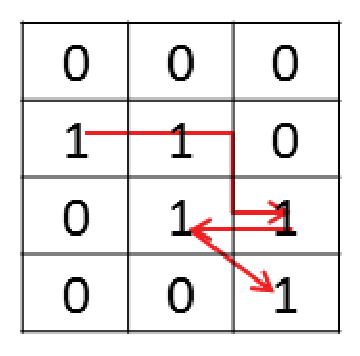
\includegraphics[width=0.1\textwidth]{images/pixOrdering2.eps}
  \label {fig:subgraph_2b}
}
\subfigure[]{
  \centering
  
\includegraphics[width=0.1\textwidth]{images/pixOrdering3.eps}
  \label {fig:subgraph_2c}
}
\subfigure[]{
  \centering
  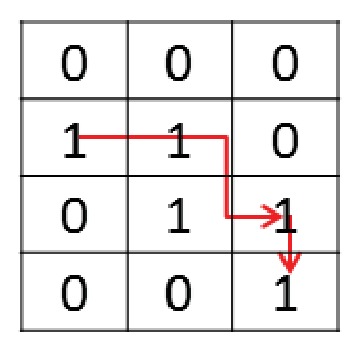
\includegraphics[width=0.1\textwidth]{images/pixOrdering4.eps}
  \label {fig:subgraph_2d}
}
\caption{Examples of edge pixels. (a) 16 pixels from the image shown in Figure2(d), where 0 is the background pixel and 1is the silhouette pixel; (b) an edge detected by the Canny operator from (a), where 1 represents edge pixels, red arrows indicate possible pixel order leading to multiple lines; (c) searching order of pixels, the middle p is the current pixel, the order of searching is labeled from 1 to 8. (d)  the revised searching order indicated by red arrows.}
\label {fig:Figure2}
\end{figure}

Let the set of edge pixels be denoted by ${P_i}, i=1,...,l$, where each pixel $P_i$ = $[P_i (x),P_i (y)]$, and $l$ is the number of pixels. The process of ordering pixels connects independent pixels ${P_i}$ according to their 8-connected neighborhood. Let the reordered pixels be placed in a $l\times2$ list $L$, where $L_1$ is the starting pixel, $L_{i+1} $is the next neighbor to $L_i$. Initially we choose an arbitrary pixel $P_k$ as the starting pixel $L_1$, set  $L_1= P_k$, and mark pixel $P_k$ as visited. Then iteratively search the next neighbor $L_{i+1}$ of $L_i$ according to the searching order given in Figure 2(c). Suppose $L_i$ is located at $p$, starting from position 1, the first unvisited $P_u$ is taken as $L_{i+1}$. The ordering process stops when the searched $L_{i+1}=L_1$. Figure 2(d) shows a revised search which avoids the polyline.
\fi


\noindent\textbf{Stroke Segmentation.} Strokes extracted from $\mathbf{I}$ can be quite long and contain a rich amount of geometric information. Modeling such a stroke as a whole entity is quite a difficult task in itself, since it should encode all possible variations that a particular stroke can take on. Instead, we resort to breaking each stroke into smaller units (called segments) that are represented in a more straightforward and conventional manner. We fit a b-spline curve to each stroke and identify break points as locations of local maximum curvature in the b-spline. We explicitly handle linear strokes by placing break points at its two ends to avoid over-segmentation. The pixels between two consecutive breakpoints (or the beginning/end of the stroke) are grouped together and denoted as a stroke segment. Figure ~\ref{fig:Figure3} shows the stroke segments extracted from two sketches taken from one of our sketch datasets.

%Figures \ref{fig:mickey} and \ref{fig:mickeyb} are examples of boundary curves with 1401 pixels and 2107 pixels from two high resolution images respectively. Curve fitting on thousands of pixels is time consuming, but high resolution images usually provide sufficient and accurate boundary and internal stroke information of the object. This is important for the SAR method because the authorship determination needs as much information as possible. To solve the time efficiency problem, we first fit a b-spline curve on pixels selected by systematic sampling from the whole pixel set $L$. Curvatures are calculated on the spline curves, and those points with local maximum curvature are selected as breaks. Then the break points will be re-located in $L$. Examples of segmentation on the boundary strokes are shown in Figure ~\ref{fig:Figure3}
\vspace{-2mm}
\begin{figure}[htbp]
\centering
\subfigure[]{
  \centering
  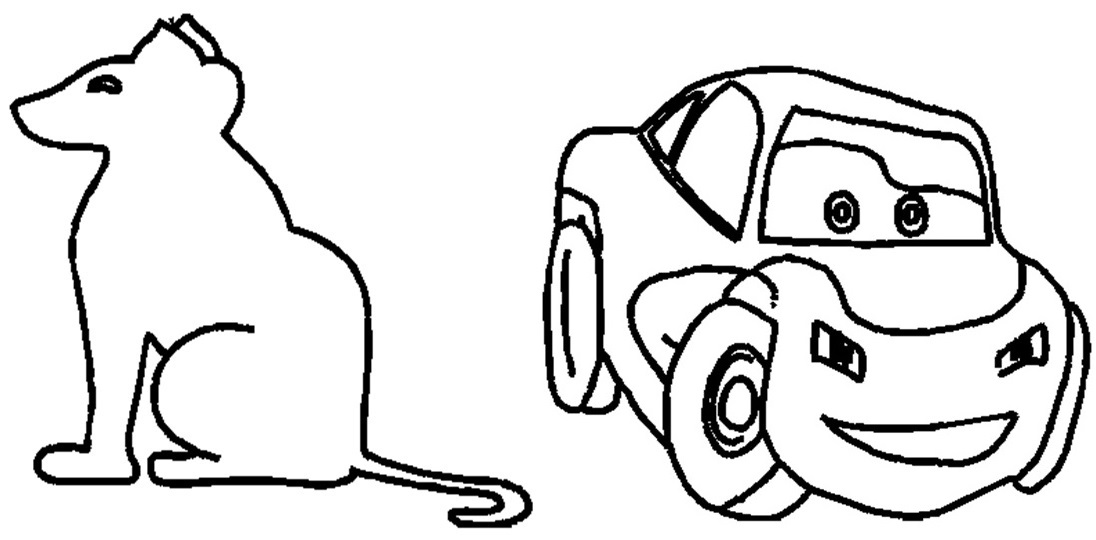
\includegraphics[width=0.21\textwidth]{images/beforeSegmantation.jpg}
  \label {fig:mickey}
}
\subfigure[]{
  \centering
  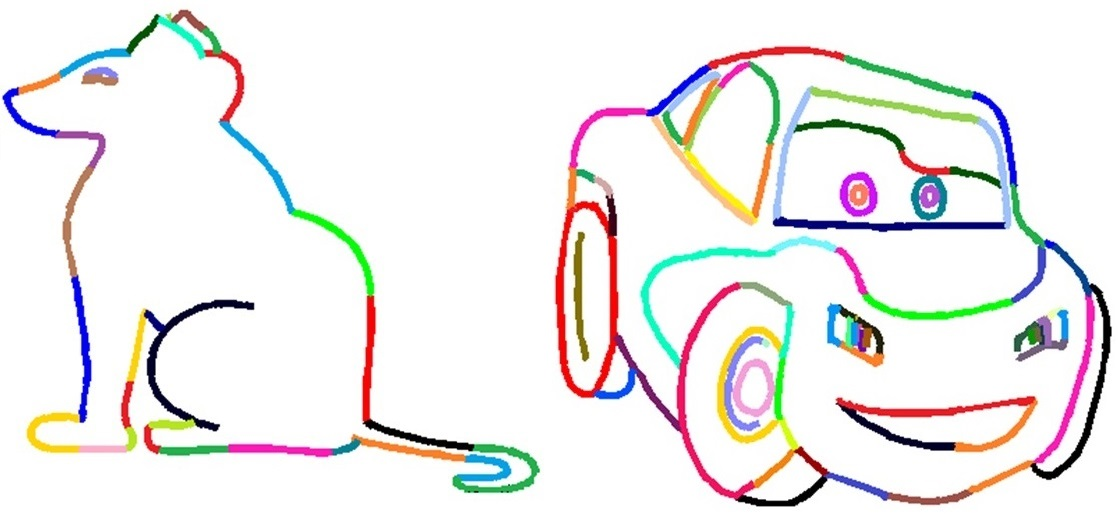
\includegraphics[width=0.21\textwidth]{images/fullSegmantation.jpg}
  \label {fig:mickeyb}
}
\vspace{-3mm}
\caption {Stroke segmentation. (a) shows two sketches after digitization and (b) shows their extracted stroke segments (color-coded)}\vspace{-3mm}
\label {fig:Figure3}
\end{figure}

% How about calling the stroke segment in this context as stroke and their union as curves or something else?

\vspace{-4mm}
\subsection{Mathematical Characterization} \label{subsec: featureExtraction}
\vspace{-1mm}
% main assumption here is that the style of an artist manifests itself in the use of particular strokes over others. We do not claim that the stroke histogram is the same across all sketches of the same artist, but we do assume that they are 'closer' to each other than to other stroke histograms. Therefore, we can find a classifier that can separate between artist sketches.
After $\mathbf{I}$ is decomposed into stroke segments, we represent it according to its stroke content.We aim to describe a stroke segment's structure and the manner in which it is drawn. We focus on local features that are simple to extract, representative, and invariant to various deformations (e.g. rotation, translation, and scale). In this paper, each segment is described by four simple features that encode eccentricity, symmetry, local consistency, and inflection. The first three features describe the stroke segment itself, while the last one describe its relationship to its adjacent neighbors. These features are both empirically validated and biologically inspired. When considering the process needed to analyze drawing traits at the stroke level, one fundamental factor arises, namely the neuro-geometry of hand-arm movement, i.e. the physiology in drawing strokes. In the foundational paper of  \cite{morasso1981spatial}, it was shown that different subjects produce hand/arm movements that are very similar to or coincide with simple curve strokes. Although low curvature change was generally maintained across different subjects and experiments, it was also found that individuals exhibited unique stroke characteristics. This finding was also confirmed in the work of  \cite{abend1982human}. In \cite{flash1985coordination}, a mathematical model based on minimizing jerk (change of curvature) and analyzing stroke velocity was verified empirically. In summary, this and other work (see references in \cite{flash1985coordination}) strongly suggest that \textbf{(1)} gesturing and strokes carry unique and identifiable aspects for an individual, and \textbf{(2)} that curvature and its change are key features for analyzing simple strokes. Inspired by the above physiological findings, we characterize stroke segments by focusing on curvature and its change in a drawn curve.

Moreover, in analyzing a large number of simple strokes, we see that a conic fit to a stroke segment is faithful to its original geometry and representative enough for the purpose of authorship recognition. From each conic, we extract eccentricity, symmetry, local consistency, and inflection features that are conveniently translation, orientation and scale invariant. Needless to say, this invariance also holds when the entire sketch is represented using stroke segment features. We give a description of these four features next.

%fit the curve’s pixels with a least squares polynomial. Among the different analytics, we looked at the evolutes of the subsequent curves (See examples, Figure. \ref{fig:evoluteofcurve}).  An evolute is the envelope of a curve’s normals. Even with high degree fits, we easily noted that evolutes of simple strokes regularly appeared to be close to the evolutes of conics as in Figure \ref{evoluteofconic}  Since conics minimize the curvature of the curve, this supported the neuro-geometry research cited above that curvature change was critical in hand/arm gestures, and it also led us to develop criteria based on 2nd order criteria, i.e. conic fits to the strokes. As an extra convenience, curvature criteria are translation, orientation and scale invariant.  This helped considerably in acquiring sample data, since information on original position, size and tilt of the drawings is not usually available for stored images.

%\SARA{Those features are both empirically derived and biologically inspired. When we considered the process needed to analyze drawing traits at the level of stroking, one fundamental factor arose is the neuro-geometry of hand-arm movement, i.e. the physiology in drawing strokes.  In the foundational paper of  \cite{morasso1981spatial} different subjects produced specified hand/arm movements that were very similar to or coincided with simple curve strokes. Although certain invariants such as low curvature change were generally maintained across different experiments, it was also found that individuals exhibited unique characteristics across a range of exercises.  The low curvature change in simple hand/arm gestures was confirmed in the thorough work of  \cite{abend1982human}, while also noting individual characteristics.  In \cite{flash1985coordination}, a mathematical model, which included stroke velocity, based on minimizing jerk (change of curvature) was verified empirically.  In total, this and other work (see references in \cite{flash1985coordination}) strongly suggest that \textbf{(1)} gesturing and strokes have unique, identifiable aspects for an individual, and \textbf{(2)} that curvature change is key for analyzing simple strokes.  We therefore characterize strokes by focusing on the individuality of curvature change in a drawn curve. Moreover, in analyzing a large variety of simple strokes, we fit the curve’s pixels with a least squares polynomial.  Among the different analytics, we looked at the evolutes of the subsequent curves (See examples, Figure. \ref{fig:evoluteofcurve}).  An evolute is the envelope of a curve’s normals. Even with high degree fits, we easily noted that evolutes of simple strokes regularly appeared to be close to the evolutes of conics as in Figure \ref{evoluteofconic}  Since conics minimize the curvature of the curve, this supported the neuro-geometry research cited above that curvature change was critical in hand/arm gestures, and it also led us to develop criteria based on 2nd order criteria, i.e. conic fits to the strokes. As an extra convenience, curvature criteria are translation, orientation and scale invariant.  This helped considerably in acquiring sample data, since information on original position, size and tilt of the drawings is not usually available for stored images.
%}

%\begin{figure}[ht]
%\centering
%\subfigure[]{
%  \centering
%  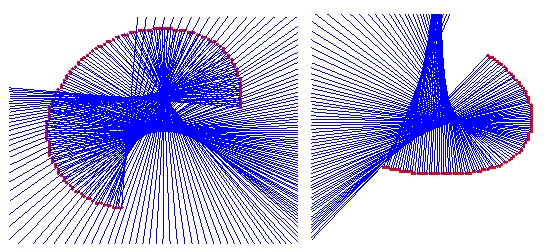
\includegraphics[width=0.26\textwidth]{images/evoluteofcurve.jpg}
%  \label {fig:evoluteofcurve}
%}
%\subfigure[]{
%  \centering
%  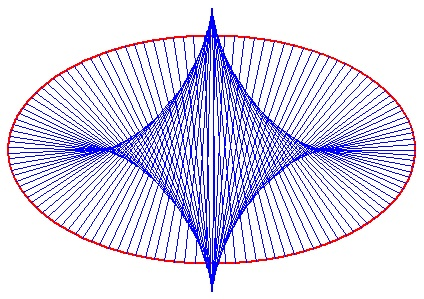
\includegraphics[width=0.18\textwidth]{images/evoluteofconic.jpg}
%  \label {fig:evoluteofconic}
%}
%\caption{(a) Evolutes of test curves (b) Evolute of a conic }
%\end{figure}
% It is worthwhile to note that other features can be used in this context, e.g. shape moments, curvature histogram, etc.

\noindent \emph{Eccentricity}: This feature represents the change of curvature in a stroke segment. It measures how the segment deviates from being circular, i.e. how rounded or sharp it is. By fitting a conic section to the stroke segment \cite{taubin1991estimation}, eccentricity ($\varepsilon$) is computed as a function of the ratio between the conic's major and minor axis lengths as in (\ref{eq: ecc}).
\vspace{-1mm}
% For example, Disney characters tend to have more rounded silhouettes using nearly elliptic curves. Compared to Disney, other cartoon companies such as Looney Tunes prefers to adorn their characters with straighter and sharper strokes.
\begin{equation}
\varepsilon=\begin{cases}
\sqrt{1-\frac{b^{2}}{a^{2}}} & \text{if the conic is an ellipse}\\
\sqrt{1+\frac{b^{2}}{a^{2}}} & \text{if the conic is a hyperbola}
\end{cases} \label{eq: ecc}
\end{equation}
\vspace{-3mm}

\noindent \emph{Symmetry}: To crudely evaluate how symmetric a stroke segment is, we simply take the absolute difference in eccentricity of the segment's two halves (refer to Figure \ref{fig:symmetry}). The segment is divided into two equal length parts (denoted as \emph{attack} and \emph{decay} following typical sketch nomenclature) and the eccentricity of each part is computed as described above.
\vspace{-2mm}

\begin{figure}[ht]
\centering
\subfigure[]{
  \centering
  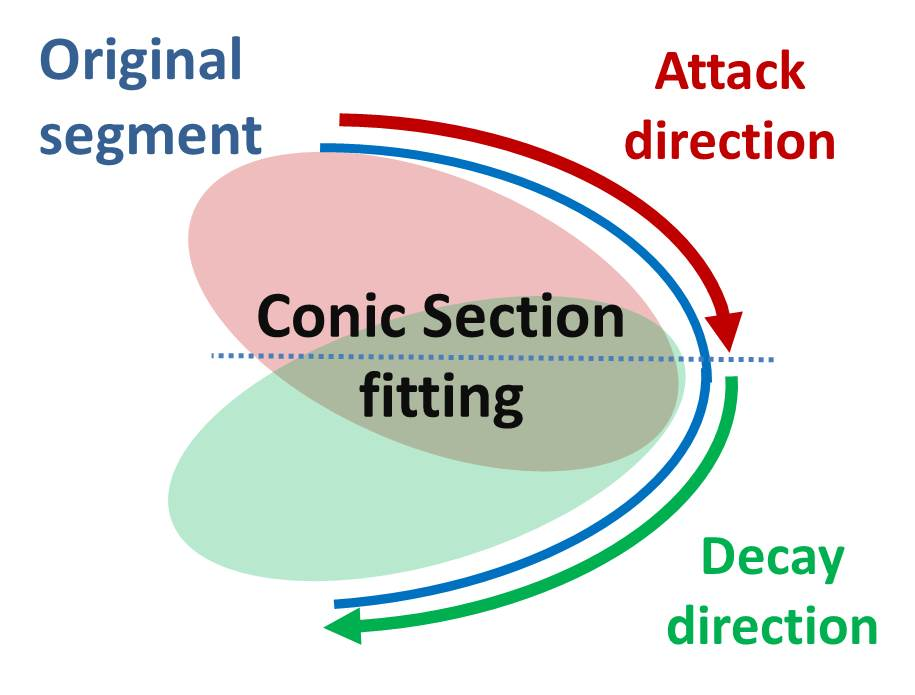
\includegraphics[width=0.18\textwidth]{images/symmetry.jpg}
  \label {fig:symmetry}
}
\subfigure[]{
  \centering
  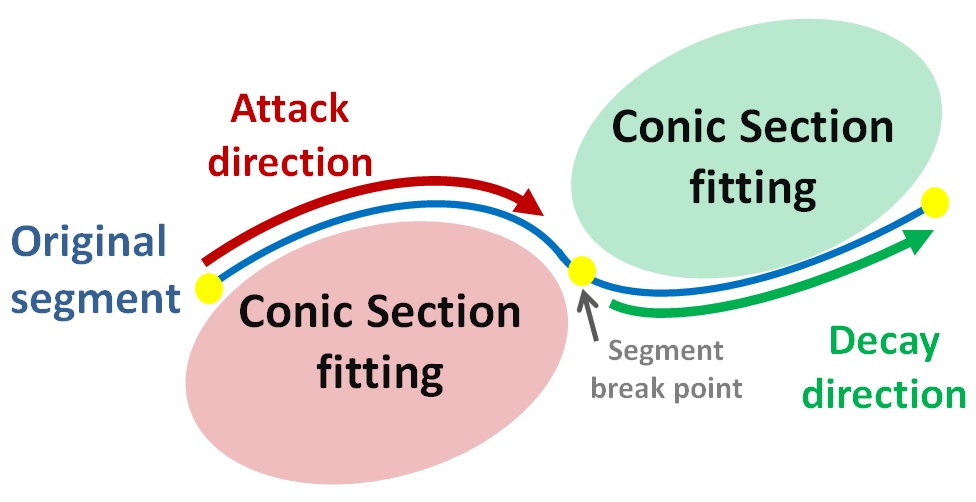
\includegraphics[width=0.26\textwidth]{images/inflection.jpg}
  \label {fig:inflection}
}\vspace{-3mm}
\caption{Attack and decay parts used to construct stroke segments. (a) shows a stroke segment divided into equal length parts enabling the computation of the symmetry feature. (b) shows two adjacent stroke segments connected by an inflection breakpoint. The inflection feature is computed by comparing these two segments.}\vspace{-6mm}
\end{figure}

\noindent \emph{Local Consistency}: This feature measures the extent of local variation within a stroke segment. It is computed as the average absolute difference between the eccentricity of the entire segment and the eccentricity of distinct overlapping parts of this segment. To generate these distinct parts, we employ a sliding window approach across the segment, where the window size is one third the size of the segment itself and the step size is half the window size. This feature captures subtle changes in shape and curvature.

\noindent \emph{Inflection}: The previous three features describe the stroke segment itself. However, characteristics of artistic style are encoded in how stroke segments are sequenced. Of special interest are locations of inflection, where the sign of curvature changes. An inflection point will be detected by SAR as a breakpoint between two stroke segments that together form a stroke (refer to Figure \ref{fig:inflection} for an example). To encode such relational information at an inflection point, we compute the absolute difference in eccentricity between each pair of stroke segments that share this inflection point. For stroke segments whose breakpoints are not inflection points, we set their inflection feature to a nominal value (-1).
%
%After we extracted a set of segments from all internal and external strokes, we fit a conic section to each curve segment. A fitted conic section can be an ellipse, parabola or hyperbola. It is an important technique in curve and surface reconstruction and has been studied thoroughly \cite{bookstein1979fitting,taubin1991estimation,zhong2007direct}. Tubin \cite{taubin1991estimation} solved the problem by minimizing the approximate mean square distance. A conic section function is given by:
%
%\begin{equation}
%Ax^2+Bxy+Cy^2+Dx+Ey+F=0,
%\end{equation}
%
%where $A$, $B$, $C$, $D$, $E$, $F$ are coefficients. The discriminant  $\Delta$, calculated by $B^2-4AC$, determines the types of conic section.  If $\Delta<0$, function (1) yields an ellipse or a circle; if $\Delta=0$, it is a parabola, and otherwise, a hyperbola. The discriminant, $\Delta$ will be set to 0 if its absolute value is less than machine epsilon 2.2204e-016 due to computation precision.
%
%Every curve segment is labeled by a specific type of conic section according to the value of $\Delta$. For different types of segments.
%
%%\noindent{\bf Local Feature Extraction.}
%After representing each curve segment with a corresponding conic section, we then calculate the eccentricity which represents the first local feature and the basis for the rest of the features. A circle has eccentricity $\varepsilon=0$, and a parabola has $\varepsilon=1$. The eccentricity of ellipse and hyperbola cannot be directly calculated by function (1). Coefficients in function (1) are converted to $(C_x, C_y, R_x, R_y, \theta)$, where $C_x$ and $C_y$ are coordinates of the center, $R_x$ and $R_y$ are the length of two axes $a$ and $b$ respectively, $\theta$ is the angle between X-axis and the major axis of the ellipse or hyperbola. Then the eccentricity $\varepsilon$ is computed by:
%\begin{equation}
%\varepsilon=\begin{cases}
%\sqrt{1-\frac{b^{2}}{a^{2}}} & \text{if} \; \Delta<0 \; (elllipse)\\
%\sqrt{1+\frac{b^{2}}{a^{2}}} & \text{if} \; \Delta>0 \; (hyperbola)\end{cases}
%\end{equation}
%
%As a general observation, using the discriminant to break down the quadratic fitting adds additional information to the process. Eccentricity reflects to what extent a conic section deviates from being circular so that the analysis of its distribution is representative of characteristics on the strokes of a shape.

%Another two local features are based on calculating the difference in eccentricity values between what we call the attack and decay parts of an artist's stroke which represent the first and the second halves of a given stroke respectively. In other words, we examine how symmetrical an artist's stroke is. The first feature of this type is applied at shoulder shaped strokes, i.e. between two break points of a segment as shown in ~\ref{fig:symmetry}. The second feature, on the other hand, is applied between the two sides of an inflection point as shown in ~\ref{fig:inflection}. The fourth and last local feature we extracted is based on comparing the difference in eccentricity values between global and local curves where global curves are the actual curve segments and local curves are portions of the global curves. We divide each global curve into 3 local curves and find the differences in eccentricity values between the local curves in comparison with the global one. {\color{red}[Mention that these features are rotation, translation, and scale invariant.][Other descriptive features (e.g. ) can be used to represent a stroke segment.]}

\vspace{-4mm}
\subsection{Feature Frequency Distribution} \label{subsec: featureExtraction}
Having each stroke segment $s_i$ of sketch image $\mathbf{I}$ characterized by the 4D feature vector of the features described above, 
this stage represent $\mathbf{I}$ as distribution of frequency of those features.


\noindent\textbf{Building a Universal Stroke Segment Dictionary.} Our assumption is that the frequency in which an artist uses particular types of strokes is a suitable indicator of his/her authorship. To formalize this observation, we compile a dictionary of stroke segments that tends to be universal among different artists. The dictionary is learned on the stroke segments of the sketches that are used in training only. To construct a dictionary of $n$ elements, we apply hierarchical k-means clustering on a large set of stroke segments. In our experiments, we set $n=60$. We denote this dictionary as the universal stroke segment dictionary as it tends to capture the most commonly used stroke segments among artists. This clustering step is first stage of the bag-of-words (BoW) model that is popularly used to represent natural images for image classification \cite{Sivic03}. We use hierarchical k-means, since it is more robust and less sensitive to the choice of $n$ than traditional k-means clustering. And it generates a tree of $n$ cluster centers (and not only a set of centers as in the case of k-means), which encodes the membership of any stroke segment at all levels of the tree and not just the leaves. To encode a stroke segment, one has to \emph{traverse} this tree starting from the root and recursively select among its children the nearest cluster center in 4D feature space. As a result, each stroke segment is encoded as a binary membership vector of length $n$, where each value reflects whether the feature traversed the corresponding tree node or not. In Figure ~\ref{fig:bagOfWords}, we show image examples of cluster centers in the universal stroke segment dictionary, as well as, the color-coded membership of each stroke segment in a sketch. Such assignment is independent of where a stroke segment exists in a sketch.


%After extracting all the local features from all the sketches, we build a visual vocabulary and for that we use a hierarchical version of k-means clustering. K-means clustering is recursively applied to compute finer and finer partitions which returns a tree where each node is a cluster center that is used to build the visual vocabulary. We choose hierarchical k-means clustering because it gave us a better visual vocabulary representation when compared against k-means clustering and visual words of regular interval values. Figure ~\ref{fig:bagOfWords} shows a sample of strokes from the dictionary of visual words along with its color coding representation on one of the sketch's silhouette.
\vspace{-4mm}
\begin{figure}[ht]
\centering
\subfigure[]{
  \centering
  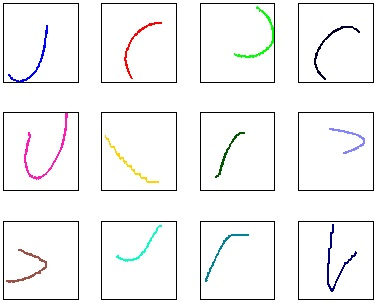
\includegraphics[width=0.24\textwidth]{images/bow.jpg}
  \label {fig:BoW}
}
\subfigure[]{
  \centering
  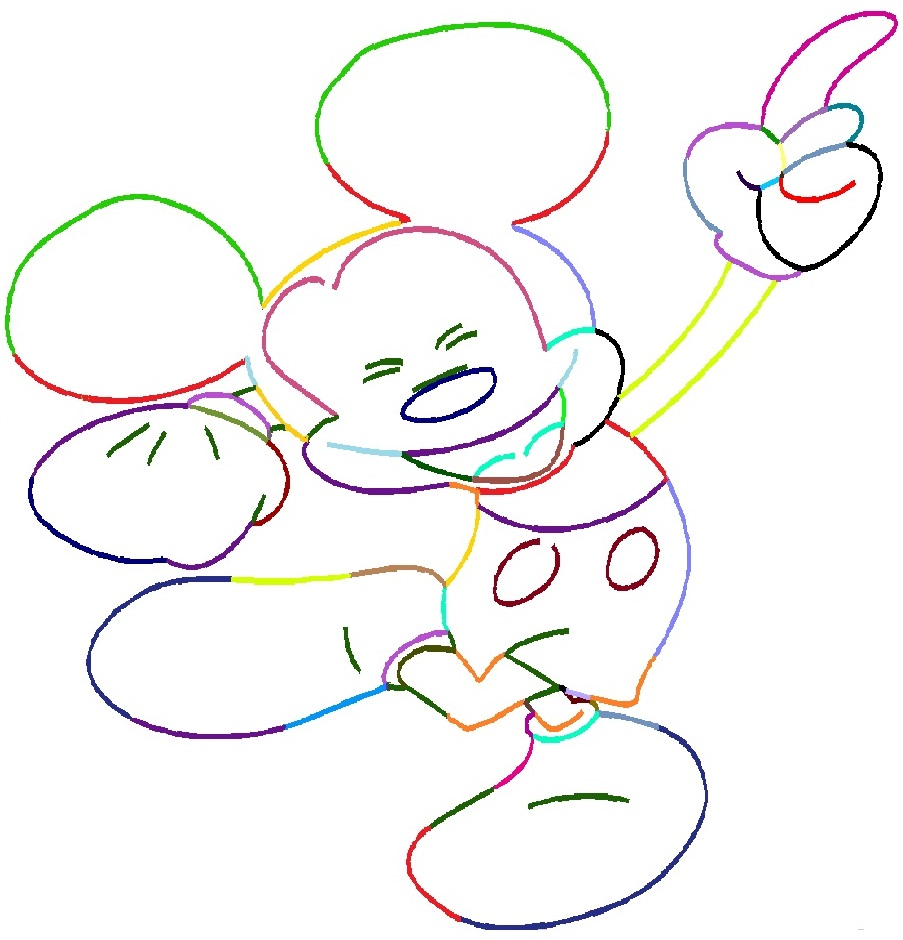
\includegraphics[width=0.20\textwidth]{images/MickyCenters.jpg}
  \label {fig:BoWSketch}
}\vspace{-3mm}
\caption{(a) Some elements of the universal stroke segment dictionary constructed from the segments of the training sketches. (b) Color-coded nearest neighbor assignment of segments to dictionary elements.}\vspace{-2mm}
\label{fig:bagOfWords}
\end{figure}

%\vspace{-2mm}
\noindent\textbf{Bag-of-Words Features.} After constructing the universal dictionary, we represent a sketch as a histogram of stroke segments following the traditional Bag-of-Words (BoW) framework. Sketch image $\mathbf{I}$ containing $m$ stroke segments produces $m$ binary membership vectors each of length $n$. These membership vectors are pooled together to produce the BoW feature vector $\mathbf{f}_{\mathbf{I}}$. We use Gaussian weighted mean pooling to encode the frequency in which an artist uses each element of the universal dictionary. As we will see, coupling $\mathbf{f}_{\mathbf{I}}$ with a discriminative model enables authorship recognition. Since the original 4 stroke segment features are invariant to rotation, translation, and scale, the BoW feature vector is invariant to these deformations \cite{lu2007survey}.


 %our bag of visual words, we use a normalized frequency histogram of visual words to represent each sketch. We apply what is called 'hard' assignment of locally extracted features to visual words \cite{Sivic03}. Such representation is what going to be used during authorship classification.

%Since the style of an artist manifests itself in the artist's use of particular stroke segments over others, representing $\mathbf{I}$

\vspace{-3mm}
\subsection{Authorship Recognition}
\vspace{-1mm}
So far, a sketch image is represented by a sparse $n$-dimensional histogram depicting the frequency in which each type of stroke segment is used by the artist in the sketch. As such, we expect the BoW feature to possess enough discriminative power to determine authorship based on simple strokes alone. We validate this assumption empirically in Section \ref{subsec:recognition}. Given a training set of sketches labelled according to the artist who drew them, we build a discriminative model using the training BoW features. In order to reduce testing time and to pinpoint the most discriminative portions of the BoW feature, we employ a forward feature selection procedure, which greedily appends a single feature at a time \emph{only} if this addition improves classification accuracy \cite{574797}. Based on our experiments, only a small subset of the $n$ features is actually used for discrimination. Using these subsampled BoW histograms, we build a multi-class classifier to assign authorship to an unseen sketch image. For sketch fraud detection, we use a binary classifier (original vs. fraudulent) instead. We experimented with a variety of classifiers and found that either an RBF (Radial Basis Function) kernel SVM or a kNN classifier can be used for this purpose. However, we decided on the kNN classifier because of its better generalizability properties and its minimal training time. We use two experimental setups to evaluate the accuracy of our classifier: 2-fold cross validation and leave-one-out. The first is a popular setup in image classification, while the latter sheds light on how dependent the classifier performance is to the amount of training data.

%\noindent{\bf Attribute Selection.}
%After Extracting all the local features all segments of a sketch, We implement a simple attribute filtering algorithm. Shall I write about this in details?

%The fourth step of SAR is to use curve features to recognize figures' authorships and classify them accordingly. Classification models are built in the new feature space, i.e. histograms of visual words. SVM and k-NN are used for categorizing objects by their authorships.

%We use nearest-neighbor classification. We find the $k$ nearest neighbors (knn) for a given histogram representation of a sketch. A histogram will belong to the category where most of the k nearest neighbors belong to. We use leave-one our and 5 fold cross validation in our experiments.


\vspace{-3mm}
\section{Sketch Datasets}\label{sec:datasets}
\vspace{-2mm}


%\begin{figure*}[htbp!]
%\centering
%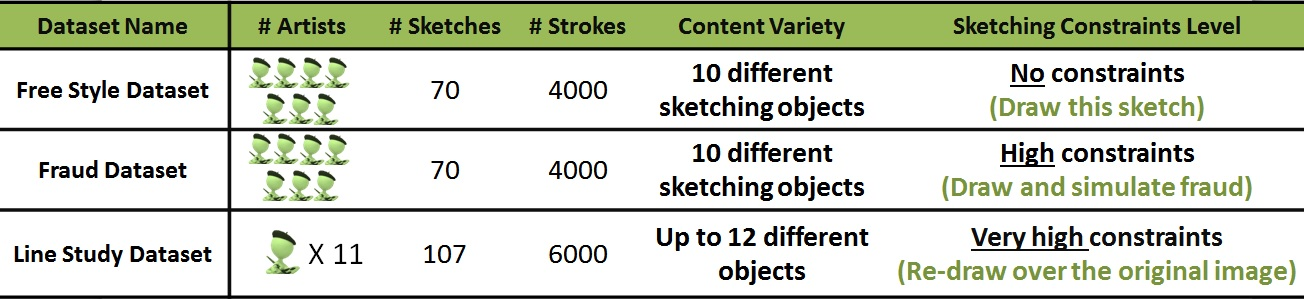
\includegraphics[width = 0.95\textwidth]{images/compDatasets.jpg}
%\vspace{-1mm}\caption {A summary of datasets used in this paper. We compiled the first two and reused the line study dataset of %~\protect\cite{Cole:2008:PDL:1360612.1360687}.}\vspace{-5mm}
%\label{datasetSummary}
%\end{figure*}


\begin{table*}[htbp!]
\begin{tabular}{|c|ccccc|}
\hline
\textbf{Dataset}                          & \textbf{\# Artists} & \textbf{\# Sketches} & \textbf{\# Strokes} & \textbf{Content Variety}       & \textbf{Sketching Constraints Level}                                                              \\ \hline
\textbf{Free Style}                       & 7                   & 70                   & 4000                & 10 different sketching objects & \begin{tabular}[c]{@{}c@{}}No constraints\\ (Draw this sketch)\end{tabular}                       \\ \hline
\textbf{Fraud}                            & 7                   & 70                   & 4000                & 10 different sketching objects & \begin{tabular}[c]{@{}c@{}}High constraints\\ (Draw and simulate fraud)\end{tabular}              \\ \hline
\multicolumn{1}{|l|}{\textbf{Line Study}} & 11                  & 107                  & 6000                & Up to 12 different objects     & \begin{tabular}[c]{@{}c@{}}Very high constraints\\ (Re-draw over the original Image)\end{tabular} \\ \hline
\end{tabular}
\vspace{-1mm}\caption {A summary of datasets used in this paper. We compiled the first two and reused the line study dataset of ~\protect\cite{Cole:2008:PDL:1360612.1360687}.}\vspace{-4mm}
\label{datasetSummary}
\end{table*}

%(e.g. the same object, the same object from different views, and different objects are sketched multiple times)
To evaluate the performance of SAR, we compile two new sketch datasets collected from experienced artists. Participating artists were screened, so as to guarantee high levels of sketching capability. The chosen artists were graphical or interior designers by profession, each with 7-10 years of sketching experience. We gave them the freedom to draw using a pen, pencil or digitally at any scale. Moreover, they were allowed to correct their strokes or redraw the entire sketch with no time limit. Since we had direct access to these professionals, we were able to administer different sketching scenarios. This allowed us to control the \emph{content variety} (i.e. what the artist draws in a sketch) and the extent of \emph{sketching constraints} (i.e. how the artist should sketch). These two factors impact the strokes an artist chooses and ultimately his/her style. To our knowledge, this work is the first to compile such a diverse set of sketch data for the purpose of studying authorship from strokes. To allow for further research in this area, we will make all these datasets (images and annotations) publicly available. Next, we describe the datasets used in this paper (refer to Table \ref{datasetSummary} for a summary).


%there does not exist an available dataset of sketches such that the same set of sketches are drawn by multiple artists who are either freely drawing without constraints or attempting to make their sketches as close as possible to the original set of sketches. With the help of a number of valued artists, we collected sketches of 3 different datasets. Participating artists have demonstrated a high level of sketching abilities through their work as some of them are graphical designers and others are interior designers and they have an average sketching experience of 7 years and a maximum of 10 years. These datasets are created such that SAR is  exposed incrementally to 3  different levels of difficulties and challenges as will be discussed in details in the following sections. We made all the sketches available as part of contribution provided in this work and we hope that interesting studies can be applied using them.
%\vspace{-2mm}
%\paragraph{Flower Dataset.} In this dataset, four different artists were provided an image of a simple flower sketch and asked to draw it multiple times as they see fit. In this case, the same object is being sketched multiple times (i.e. the content variety is minimal). Moreover, artists were given complete freedom to draw the assigned sketch without any constraints or specific instructions. We will see that this constraint-free type of sketching allows artistic style to be more distinguishable among different artists than constraint-ridden sketching, of which sketch fraud is a prime example. This dataset will be the first test of SAR's ability to determine authorship from sketched strokes alone.

%constrained sketching tasks and thus experimenting using this dataset is considered to be the first milestone to test the performance of SAR.
%\vspace{-2mm}
%\paragraph{Character Dataset.} Unlike the previous dataset, artists in this dataset were asked to sketch the same cartoon character viewed from 12 distinct viewpoints. We chose Mickey Mouse, a famous Disney character, because it is a well known character and relatively easy to sketch. Artists were encouraged to draw as close as possible to the cartoon images given to them and no further instructions were given. This dataset clearly presents a higher level of challenge as compared to the flower dataset, especially since content variety here is significantly higher.

%Using this dataset, SAR is exposed to a higher level of challenge compared to the previous flower sketches because as the level of sketching constraints assigned is slightly higher and there is more content variety. i.e. we attempt to identify the authorship of a sketch by comparing it to a different content.

%We first collected the different views of Mickey images over the web and we asked 3 different artists to sketch them.

%\vspace{-2mm}
\noindent\textbf{Free Style Dataset.} We collected 10 images of objects from diverse semantic categories and then asked 7 artists to sketch them. The objects were chosen to be detailed enough to adequately reflect artistic style and to be relatively easy to replicate by an experienced artist in a reasonable amount of time. The 70 sketches (10 from each artist) were collected in three weeks. No constraints or specific instructions were given to the artists, thus, giving them complete sketching freedom. 
%We will see that this constraint-free type of sketching allows artistic style to be more distinguishable among different artists than constraint-ridden sketching, of which sketch fraud is a prime example. %This dataset will be the first test of SAR's ability to determine authorship from sketched strokes alone.


%\vspace{-2mm}
\noindent\textbf{Fraud Dataset.}  Here, we simulate a sketch fraud scenario. Using the same images in the free style dataset, we chose the sketches of one of the artists as \emph{original} drawings. We asked the other 6 artists to draw all the original sketches. We provided them with an instruction sheet, where they were requested to draw the original sketches in such a way that it would be very hard to distinguish their \emph{own} drawings from the originals, thus, simulating sketch fraud. The 6 artists were prohibited from using methods or supplies (e.g. translucent tracing paper) that could produce copies of the original sketches. Over a period of 2 weeks, we collected a total of 60 sketches. (refer to Figure \ref{FraudDataset} for examples). Since the artists were requested to simulate sketch fraud, this dataset is highly constrained from an artistic style perspective. Therefore, it poses a substantial challenge to any authorship recognition system, albeit manual or automatic.

\begin{figure*}[htbp!]
\centering
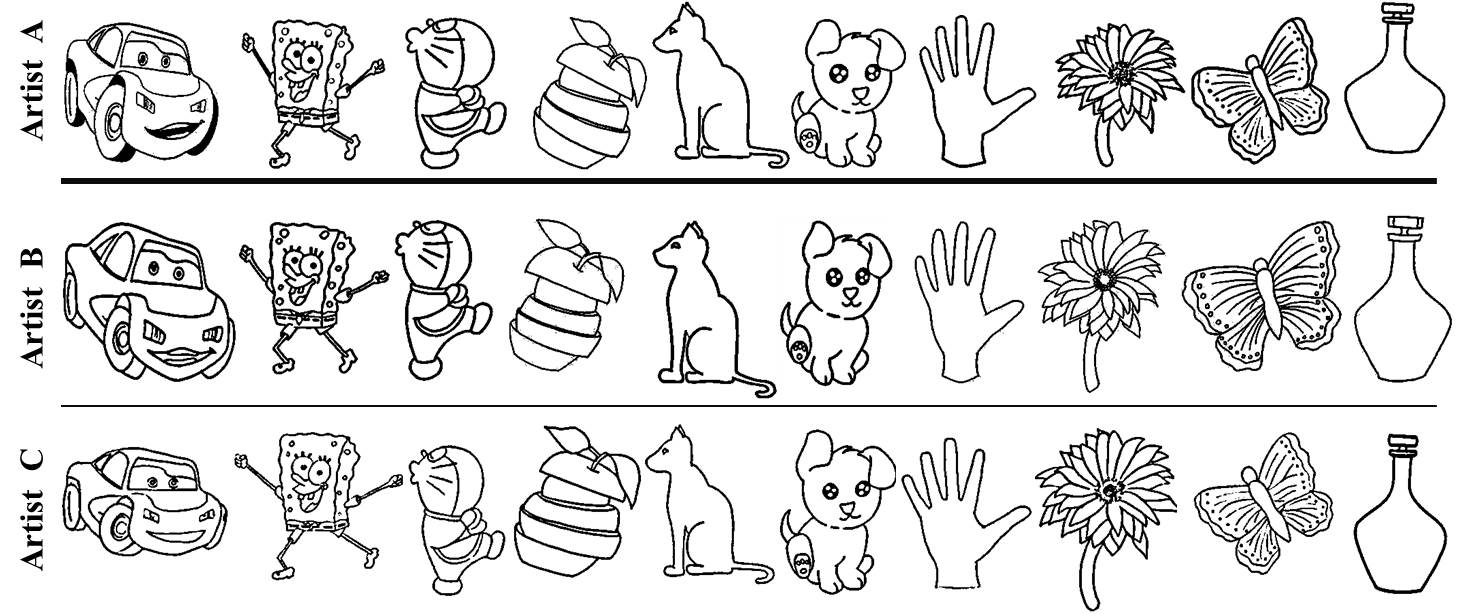
\includegraphics[width = 1.0\textwidth]{images/fraudExperiment.jpg}
\vspace{-6mm}\caption {Samples of sketches from the fraud dataset. The first row shows the original sketches drawn by Artist A. The other three rows show the sketches of 2 other artists (Artists B and C), who attempted  sketch fraud. Obviously, the \emph{fraudulent} sketches look extremely similar to the originals, making authorship recognition (manual or automatic) quite difficult.}\vspace{-5mm}
\label{FraudDataset}
\end{figure*}

%In this dataset, we simulate a sketch fraud scenario. We first collected 10 objects of various semantic categories and asked one of the participating artists to sketch them. From a fraud perspective, these 10 sketches can be considered to be \emph{original} drawings. The objects were chosen to be detailed enough to adequately reflect the artists' sketching style and to be relatively easy for any experienced artist to replicate in a reasonable amount of time. After the originals were generated, we tasked 6 other artists to draw them. Along with the original sketches, we provided them with an instruction sheet, in which we asked them to draw the provided sketches such that it would be very hard to distinguish their \emph{own} drawings from the \emph{original} ones, thus, simulating sketch fraud. The 6 artists were prohibited from using methods or supplies (e.g. translucent tracing paper) that would enable them to produce copies of the original sketches. Over a period of 2 weeks, we collected a total of 70 sketches from the 7 artists. Some sample sketches are shown in Figure \ref{FraudDataset}. Since the artists were requested to simulate sketch fraud, the generated dataset is considered highly constrained and significantly diverse in content. It poses a substantial challenge to any authorship recognition system, albeit manual or automatic.


%compiled a fraud experiment which we conducted with the aim to experiment SAR on a variety of datasets types and to expose our techniques to different levels of challenges to assess its effectiveness and value. In our experiment, we first collected 10 subjects under various categories to be sketched initially by one of the collaborating artists in our experiment.

%The subjects are chosen such that they are detailed enough to adequately reflect the artist's sketching style under different sketching subjects and to be considerably easy for any artist to replicate and not time consuming as well.

%In the next stage of the experiment, we assigned 6 other artists to draw the sketches provided by the first artist. Along with the sketches, we provided them with an instruction sheet in which we asked them to sketch the assigned sketches such that it is hard to distinguish their drawings from the original ones so that they simulate a sketching fraud attempt.

%Moreover, they were allowed to correct their strokes or redraw the entire sketch if they needed we assigned no time limit for them to draw.

%Artists, on the other hand, were encouraged to use strong, dark and smooth lines, be especially accurate to make the sketches very similar to the presented sketches and were prohibited to copy the sketches.

%Towards the end of the experiment which expanded for a period of 2 weeks, we collected a total of 70 sketches provided by 7 artists. A sample of these sketches is in figure ~\ref{FraudDataset}.

%Given that artists were requested to simulate a fraud attempt while sketching the assigned subjects, we consider the sketching task for this dataset to be highly constrained and thus more challenging to SAR than the previous 2 datasets.




%\vspace{-2mm}
\noindent\textbf{Line Study Dataset.} We also use the line study dataset generated in \cite{Cole:2008:PDL:1360612.1360687}. This dataset is a collection of sketches of various objects (e.g. mechanical tools, automobile parts, and bones) drawn by multiple artists. The sketching tasks were highly constrained, since artists were asked to draw their sketched lines over a faded copy of the original image. Clearly, the task of recognizing sketch authorship in this dataset is more difficult than the previous two. We selected all sketches from artists, who drew at least 6 sketches, thus, leading to a dataset of 107 sketches from 11 artists.  %Given such highly constrained sketching tasks, we want to experiment the performance of SAR and compare this against.
%{\color{red} [Put a reference next to the Line Study dataset]}

%Figure ~\ref{datasetSummary} provides a summary of all the datasets described above.


\vspace{-3mm}
\section{Human Sketch Authorship Recognition}\label{sec:humanexps}
\vspace{-2mm}
For comparison and as a baseline, we study the inherent difficulty of the authorship recognition problem for humans. The human visual system (HVS) is renowned for its effectiveness in successfully completing many high-level recognition tasks (e.g. object and action recognition), so much so, that it remains the \emph{gold standard} to which automated recognition systems aspire. Despite significant advances in computer vision, the HVS almost always outperforms automated methods in such tasks. However, there \emph{do exist} recognition tasks, in which the HVS underperforms. These tasks usually deal with \emph{fine-grained} recognition of objects (e.g. faces), where the inter-class variation is minimal and on par with the intra-class variation. We motivate this fact with an example. Although the HVS can easily discriminate between a 'chair' and a 'dog', it does not do so well in recognizing a person's face in a large dataset of people (e.g. the entire population of a country) from the same cultural and racial background. The differences between people's faces are so subtle that the minute details discriminating them cannot be uncovered by the HVS. However, it is exactly these details that automated recognition methods focus on. This enables them to outperform the HVS in these tasks (e.g. robust face recognition \cite{4483511}). In this section, we provide extensive empirical evidence from two user studies that highlight the sheer difficulty people and experienced artists face when trying to recognize authorship from 2D sketches.% (similar to fine-grained face recognition).

%The first was announced to the public while the second one was targeting just a sample of the artists community. The 2 user studies are discussed in details below. Later in this paper, we will show how SAR outperforms human and artists in distinguishing the authorship and originality of sketches.

%In this section, we analyze human and artists sketch authorship recognition performance. For this purpose, we conducted 2 user studies where the first study was announced to the public while the second one was targeting just a sample of the artists community. The 2 user studies are discussed in details below. Later in this paper, we will show how SAR outperforms human and artists in distinguishing the authorship and originality of sketches.


%\vspace{-2mm}
\noindent\textbf{Authorship Recognition by Non-artists.} The aim of this study is to shed light on how accurately people can recognize sketch authorship. As an online quiz, participants are first shown sample sketches from the free style dataset labled with artists who drew them. We showed 5 randomly selected sketches from each of the 7 artists. Next, we administered for each online participant a total of 5 questions, each of which asked him/her to assign an \emph{unseen} sketch to one of the 7 artists that he/she thought drew it. We chose to show users only 5 of the 10 images per artist so as not to overwhelm them. We allowed participants to zoom-in to the images when needed. To reach a large number of participants, we published our user study on Amazon Mechanical Turk (AMT). To validate the quality and seriousness of each Turker's answers (as usually done in practise), we administer a control question at the beginning of the quiz. Moreover, Turkers are randomly directed to one of the many versions of the online study and answers from unique workers are recorded.

% This study included more than a 1000 participants.
After two months of activity and more than 2000 unique participants, the accumulated results of this study show that people can successfully recognize the authorship of a sketch (among 7 different artists) with an average accuracy of 36\% and with standard deviation of 10\%. Participants took an average of 4 minutes to complete the assigned quiz. From this result, we see that average human performance is only moderately better than a random choice classifier (i.e. choose one of the 7 artists at random irrespective of what the sketch is), which has an average accuracy of 14\% in this case. Obviously, this establishes that sketch authorship recognition is quite difficult for people. More importantly, we show later in this paper that our automated SAR approach achieves an average accuracy of 60\% under the same conditions.

%These results indicate that providing people and professionals with a tool that will assist them in distinguishing authorship of similar sketches is of an added value and an extension to an average human ability.


%\vspace{-2mm}
% might want to add that this is why fraud is hard to catch. Humans cannot even do it.
\noindent\textbf{Sketch Fraud Detection by Artists.} Similar to the previous study, but targeting artists specifically, since it is conceivable that the average person might find this task difficult due to his/her lack of sketching experience and/or artistic talent. The aim here is to evaluate the performance of artists in discriminating fraudulent sketches from original ones. A total of 25 experienced artists were given an online quiz, where 5 original and 5 fraudulent sketches were made known to each user. The sketches were taken from the fraud dataset described earlier. Each artist is then given a set of 5 recognition questions, whereby he/she needs to label the unseen sketch as original or fraud. Moreover, artists were given the chance to view their quiz results and to email us feedback. Again, not all the images in the dataset are shown to the online users so as not to overwhelm them.

The quiz results show that the artists could distinguish original sketches from fraudulent ones only 52\% of the time, as compared to 50\% random chance. Each artist took an average of 5 minutes to complete the task. As expected, most of the feedback we received elaborated on how truly difficult the task was. Later, we show that SAR significantly outperforms the artists' recognition accuracy, thus, motivating the plausibility of using SAR in an automated fraud detection system for sketches (e.g. patent drawings and cartoon sketches). We include links to both quizzes in the \textbf{supplementary material}.
%Knowing that experienced artists found such distinction difficult then we believe SAR is needed to offer a new automated solution to such a challenge.


\vspace{-3mm}
\section{Experimental Results and Evaluation}\label{sec:exp}
\vspace{-2mm}
This section presents a number of experimental results we obtained to assess multiple facets of the proposed SAR approach. \textbf{(1)} To evaluate the effect of sketching constraints on SAR, as well as, its overall effectiveness in recognizing sketch authorship and detecting sketch fraud, we test SAR on the datasets described in Section \ref{sec:datasets}. \textbf{(2)} We also evaluate the sensitivity of SAR to a number of algorithmic variations. These results, in turn, are used to design the most representative and discriminative variant of SAR. %We believe that this analysis will assist other researchers in developing their own methods for stroke authorship recognition. %\textbf{(3)} To empirically validate the difficulty of the problem at hand, we conduct extensive user studies that establish grounds for comparing human recognition performance to that of SAR.

\vspace{-2mm}
\subsection{Computational Authorship Recognition}\label{subsec:recognition}
\vspace{-2mm}
We ask the following questions: Are simple strokes unique to the artist who draws them?  If they are, then to what extent can they identify the author who drew them? To our knowledge, these questions are not adequately addressed in prior work. To answer them, we conduct several experiments on three separate datasets, which provide a rich diversity of sketch content and sketching constraints. In what follows, we report SAR classification accuracy for each dataset and provide cross-dataset analysis. We also evaluate SAR's ability to detect sketch fraud using the fraud dataset.

%\paragraph{Flower Dataset.} This dataset is created by asking 4 artists to draw the same sketch of a flower multiple times without imposing any other instructions or constraints. SAR authorship classification accuracy on test data for this dataset is 96\% and 88\% using leave-one out and 5-fold cross validation respectively with 15\% standard deviation. For comparison, a random choice classifier in this case has an average accuracy of 25\%.

%\paragraph{Character Dataset.} In this dataset, the same character (at 12 different viewpoints) is drawn by 3 different artists. Similar to the flower dataset, artists were given the freedom to draw the cartoon character as they saw fit. SAR accuracy in this case is 87\% (leave-one) and 83\% (5-fold cross validation) with a standard deviation of 12\%. This accuracy is significantly higher than random chance (i.e. 33\%).
%\vspace{-3mm}
\noindent\textbf{Free Style Dataset.} On this constraint-free dataset, SAR accuracy on test data is 60\% and 57\% using leave-one out and 2-fold validation respectively with 8\% standard deviation. For comparison, random chance in this case is 14\%.

%As mentioned earlier, we compiled this dataset by asking 7 different artists to draw 10 different objects that are of various semantic meanings without imposing any other instructions or constraints. SAR authorship classification accuracy on test data for this dataset is 60\% and 57\% using leave-one out and 5-fold cross validation respectively with 8\% standard deviation. For comparison, a random choice classifier in this case has an average accuracy of 14\%.
%\vspace{-3mm}
\noindent\textbf{Fraud Dataset.} Is artistic style among different artists still preserved when they are consciously attempting to commit fraud? To answer this, we use our fraud dataset to build a 7-class SAR classifier to discriminate among the 7 artists. Using this dataset, random chance is 14\%. Here, SAR reaches a significantly higher average accuracy of 51\% (leave-one-out) and 45\% (2-fold cross validation) with 9\% standard deviation. This result suggests that an artist's sketching style is still distinguishable (to a certain extent) even when attempting sketching fraud. To visualize the discrimination power of SAR, we show the BoW features of three sketches (same object) drawn by 3 artists from this dataset in Figure \ref{HistogramsComparisonFraud}. One of the sketches is an original and the rest are fraudulent. Although all three sketches look very similar, their underlying features have obvious differences, which SAR capitalizes on to determine authorship.\\


\vspace{-4mm}
\begin{figure}[!htb]
\centering
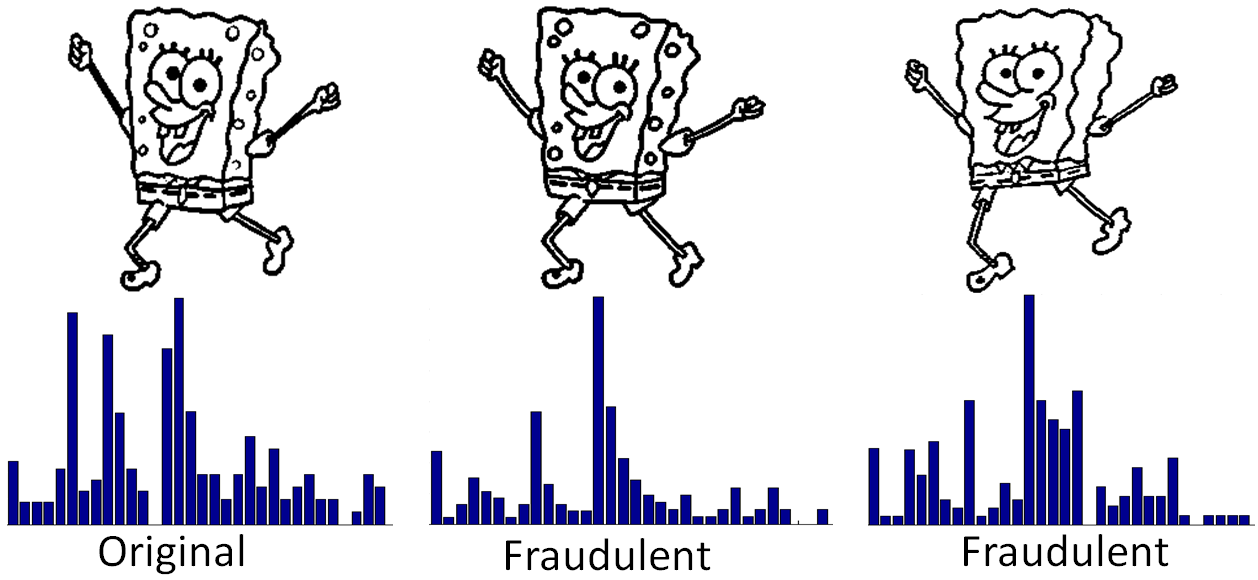
\includegraphics[width = 0.5\textwidth]{images/HistogramsComparisonFraud3.png}
\vspace{-5mm}\caption{BoW features of the same sketch object drawn by 3 artists (one original and two fraudulent). Although they look very similar, their features are different.}
\label{HistogramsComparisonFraud} \vspace{-4mm}
\end{figure}



%in an open case (i.e. the fraudulent identity is not known), which is usually the scenario in reality. For this purpose, we entirely exclude one set of fraudulent sketches by one of the artists from the training samples and used that as our test. For the training part, we have gradually increased the number of fraudulent sketches, starting by 10 sketches and ending with 50 sketches. This is along with the original sketches. Average binary classification accuracy results as the number of training samples increases are shown in Figure \ref{fraudResults}. Results have shown that  the more we train SAR on what is not original, the better its ability gets in detecting an external fraudulent sample to reach up to 96\% classification accuracy when 50 fraduelant sketches are used in the training.  Overall we conclude that espite the extremely high similarity between fraudulent and original sketches, SAR is able to effectively spot fraud. In fact, this sheds light on SAR's applicability and usefulness in the field of artistic fraud detection. \SARA {One could say this is due to the increased probability of detecting the fraudulent sketches with non-balanced binary classes (discuss with Bernard)}

%This dataset has a different setup than the previous ones. A set of 6 artists were asked to simulate an attempt at sketching fraud by drawing a set of sketches labeled as \emph{originals}, which were drawn by a $7^{\text{th}}$ artist. They were specifically instructed to make their own drawings  considerably hard to distinguish from the original ones. This experiment aims to evaluate SAR's ability to detect fraud in a realistic scenario.

%65\% - 73\% - 78\% - 86\% - 96\%
%There are 10 original sketches and 60 fraudulent ones in total, which leads to a substantially unbalanced dataset.

%Special care was taken in training (e.g. dataset downsampling and sample pruning), so as not to artificially bias the SAR classifier to the fraudulent class that contains much more samples than the original class. As a result, SAR successfully detects fraudulent sketches with an accuracy of 95\% (leave-one out) and 92\% (2-fold cross validation) and with a standard deviation of 14\% . Despite the extremely high similarity between fraudulent and original sketches, SAR is able to effectively spot fraud. In fact, this sheds light on SAR's applicability and usefulness in the field of artistic fraud detection.

%Thus, we have 2 groups, one contains the original sketches and the other contains the fraudulent ones and it has much more number of sketches than the ones in the original. To avoid falling into classifying non-balanced data, we randomly selected the same number of sketches as in the original sketches from the pool of fraudulent sketches so that equal classification chances are assigned to test data.


%\vspace{-2mm}
\noindent\textbf{Line Study Dataset.} The sketching task in the dataset compiled by ~\cite{Cole:2008:PDL:1360612.1360687} is highly constrained as discussed in Section \ref{sec:datasets}. As it is similar in spirit to the fraud dataset, we expect similar results. We train and test SAR in the same way as before but with a total of 11 artists and 107 sketches. With 11 classes, random chance is 9\%, which is significantly lower than SAR's average accuracy of 33\% (leave-one out) and 30\% (2-fold) with 7\% standard deviation. This noteworthy discrepancy in performance indicates that artists still maintain some uniqueness in their sketching style, even though they are forced to copy a different style altogether.

We give a performance summary for SAR on the three datasets in Table ~\ref{table:accuracy}. The slight difference in accuracy between leave-one out (i.e. all but one sketch are used for training) and 2-fold cross validation (i.e. only 50\% of sketches are used for training) indicates that SAR is reasonably insensitive to the amount of training data used. This also suggests that SAR is generalizable, a promising property for a classifier in the presence of unseen data.

%\begin{table}[htbp!]
%\caption {A summary of SAR performance on three datasets. Average accuracy is reported for leave-one-out and 2-fold setups. Random chance accuracy and the number of classes are also provided.}
%\label{table:accuracy}
%\vspace{-2mm}
%\centering
%\small
%\begin{tabular}{p{1.1cm} p{0.5cm}  p{0.7cm} p{1.4cm} p{1.0cm} p{0.3cm}  }
%& Num classes & Random Choice \% & Leave-One Out \% & 2-Fold  \% & std \% \\ \hline

%Free Style           & 7 & 14 & 60 & 57 & 8 \\
%Fraud                & 7 & 14 & 51 & 45 & 9\\
%Line Study           & 11& 9  & 33 & 30 & 7\\
%\end{tabular}
%\end{table}

\begin{table}[htbp!]
\caption {A summary of SAR performance on three datasets. Average accuracy (\%) is reported for leave-one-out and 2-fold setups. Random chance accuracy (\%) is also reported for comparison.}
\label{table:accuracy}
\vspace{-2mm}
\centering
\small
\begin{tabular}{cccccc}
&Rand Chance &Leave-one out & 2-Fold &std \\ \hline

Free Style           & 14 & 60 & 57 & 8\\
Fraud                & 14 & 51 & 45 & 9\\
Line Study           & 9  & 33 & 30 & 7\\
\end{tabular}
\end{table}

%\vspace{-2mm}
\noindent\textbf{Cross-Dataset Analysis.} In the datasets above, the contributing artists were subject to varying levels of sketching constraints, ranging from unconstrained (free style dataset) to highly constrained (line study dataset). To investigate the sensitivity of SAR performance with sketching constraints, we compare its accuracy across all datasets in Figure ~\ref{crossDatasetsPlot}. The datasets are ordered in increasing levels of constraint. To normalize the effect of different numbers of classes across datasets, we plot the ratio of SAR accuracy to random chance. As expected, recognizing sketch authorship becomes harder as more constraints are imposed on the artist. However, on all the datasets, SAR performance is significantly (at least 2.5 times) higher than random chance. This suggests that artists do \emph{not} lose all characteristics of their unique style even under the strictest of constraints.

%a comparison between SAR performance across all datasets, so as to investigate how the uniqueness of artistic strokes is influenced by imposing more control and adding more constraints on the sketching process. In Figure ~\ref{crossDatasetsPlot}, datasets are ordered in increasing amount of constraint. As might be expected, the recognition performance (w.r.t. to random chance) is inversely proportional to the amount of constraints imposed. From this experiment, we are lead to two main conclusions. First, the more freedom artists are given during the sketching process, the more likely their unique artistic style will be preserved. Second, even with highly constrained sketching tasks such as sketching fraud, artistic strokes maintain a certain level of uniqueness and discriminability.

\begin{figure}[htbp!]
\centering
\subfigure[]{
  \centering
  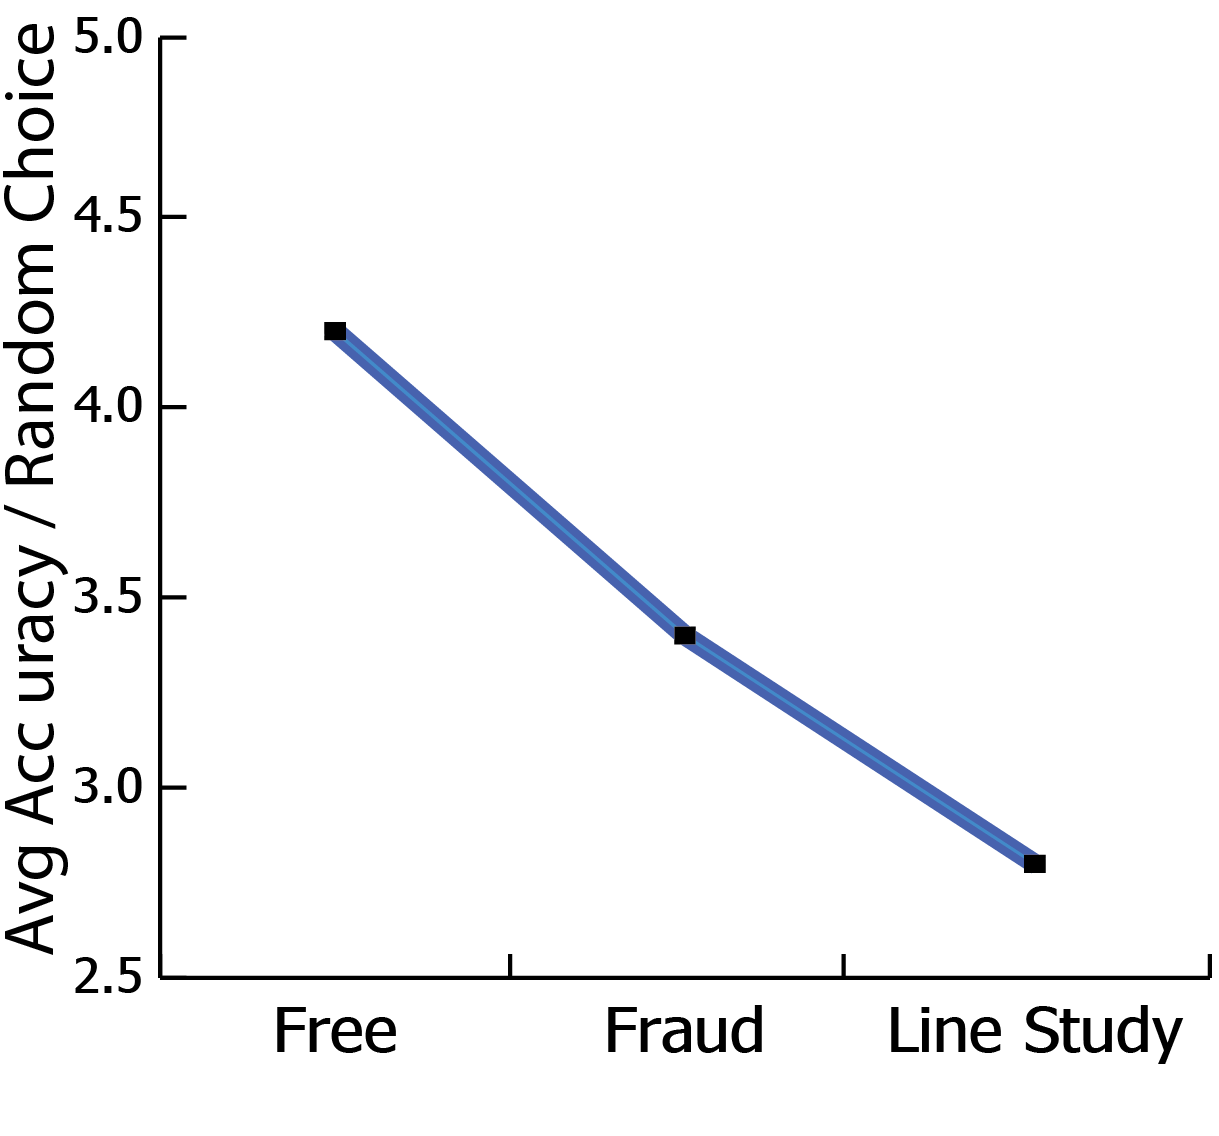
\includegraphics[width=0.225\textwidth]{images/sketchConstraints.png}
  \label {crossDatasetsPlot}
}\hspace{-3mm}
\subfigure[]{
  \centering
  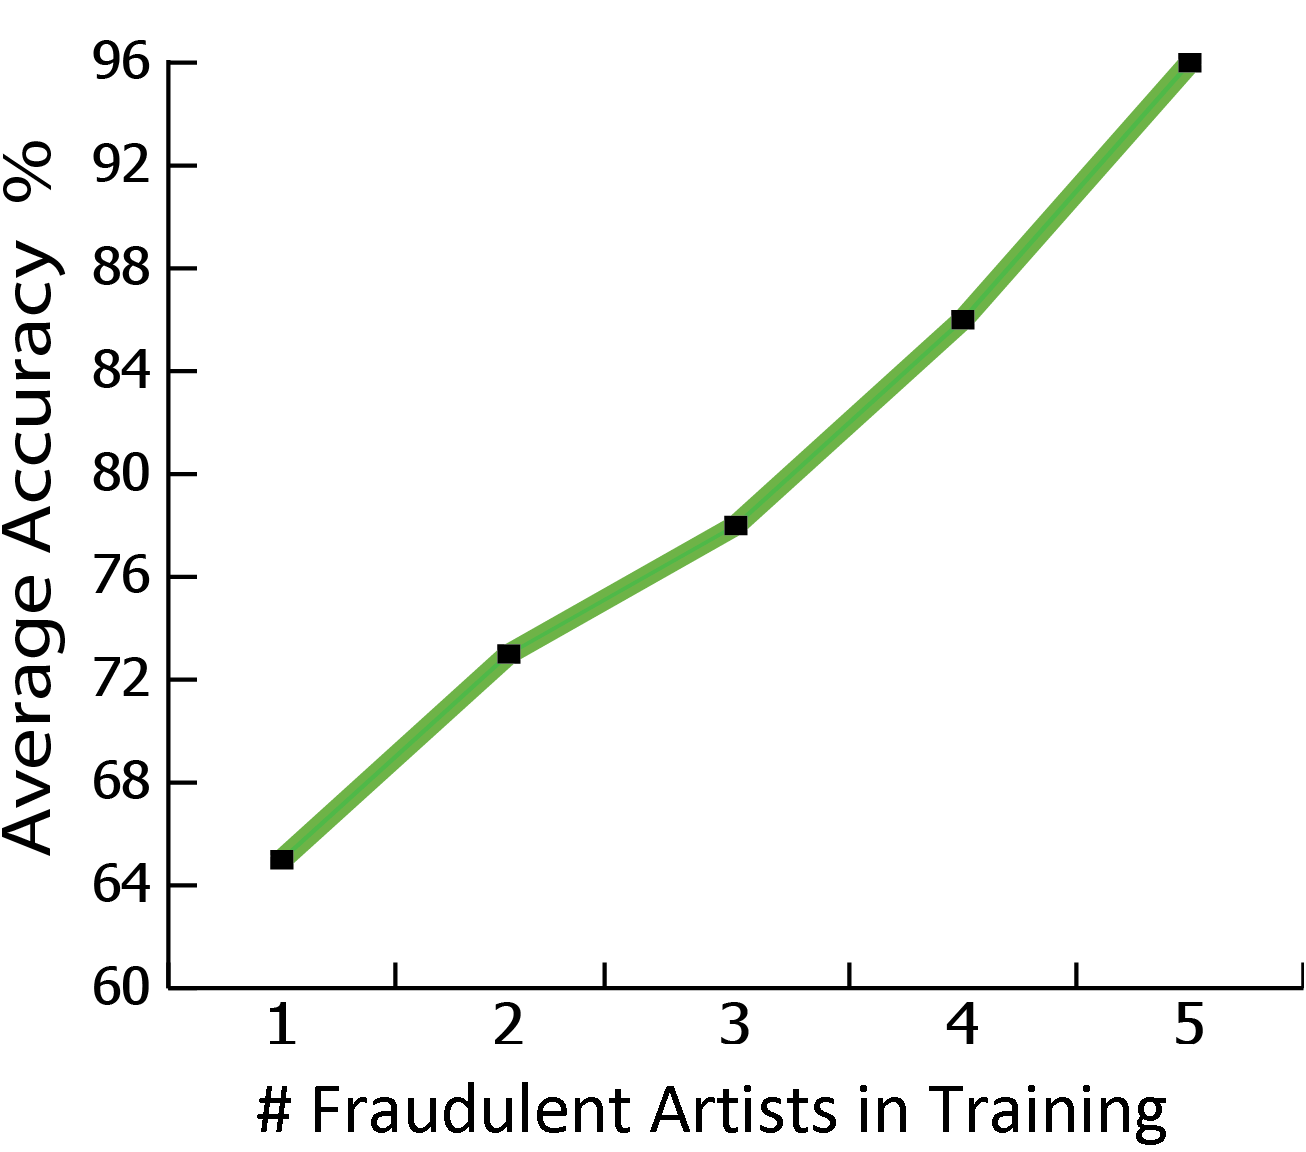
\includegraphics[width=0.225\textwidth]{images/fraudResults.png}
  \label {fraudResults}
}
\vspace{-2mm}\caption{(a) The ratio between SAR accuracy and random chance on three datasets organized in increasing order of sketching constraints. Clearly, the more constraints imposed on artists, the less discriminative their strokes become. (b) Fraud recognition performance improves as more fraudulent artists are used in training, especially on sketches from artists who were not included in training.}\vspace{-3mm}
\end{figure}


\begin{figure*}[htbp!]
\centering
\subfigure[]{
  \centering
  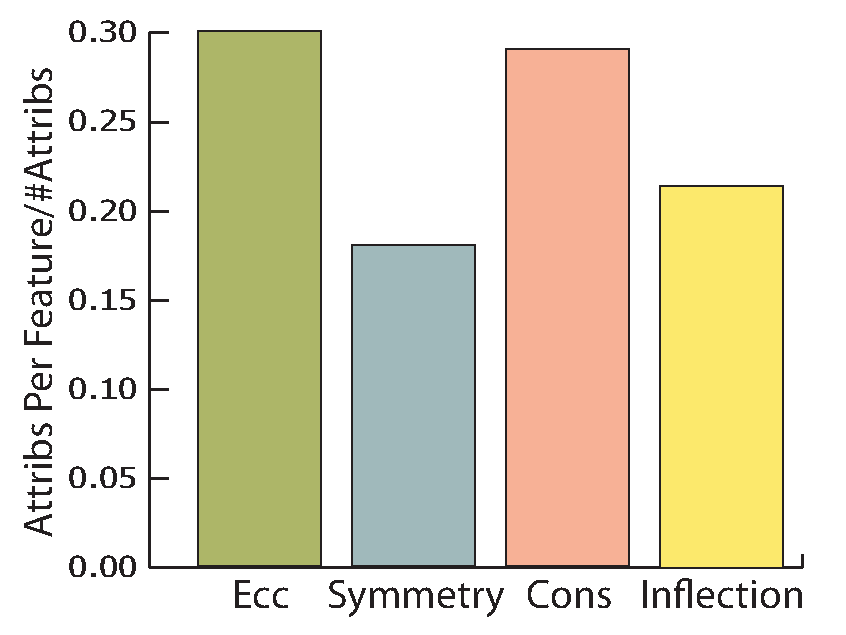
\includegraphics[width=0.35\textwidth]{images/FeatureTypeCont}
  \label {FeatureTypeCont}
}
\subfigure[]{
  \centering
  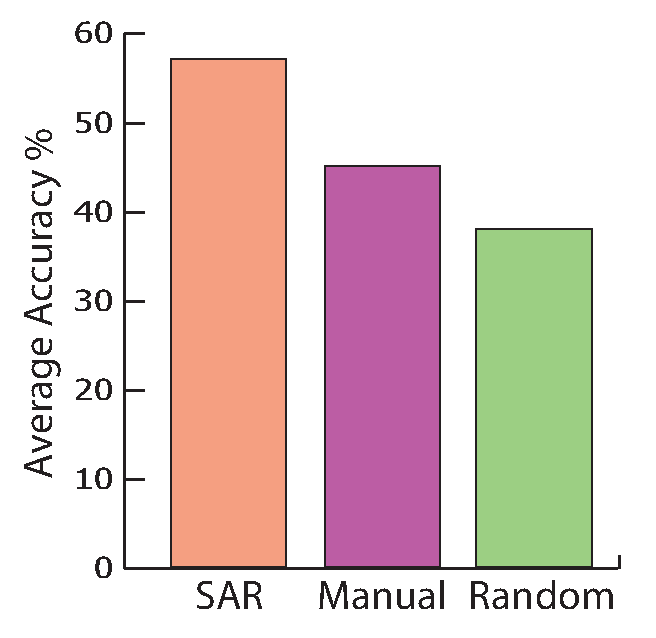
\includegraphics[width=0.27\textwidth]{images/segAlg}
  \label {segAlg}
}
\subfigure[]{
  \centering
  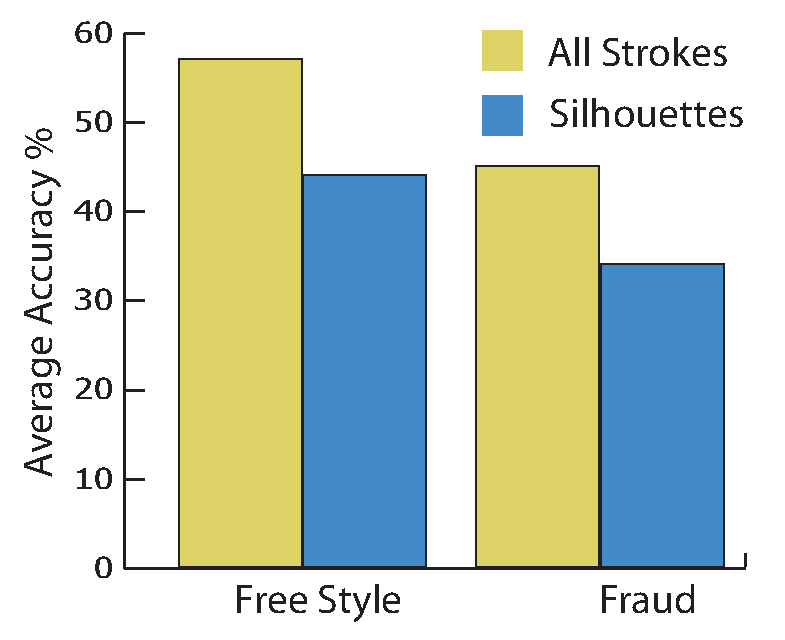
\includegraphics[width=0.32\textwidth]{images/sillVsInternal}
  \label {silAssesPlot}
}
\vspace{-4mm}\caption{(a) Contribution of each feature type to SAR recognition. (b) SAR accuracy on the free style dataset when its segmentation method is replaced with a manual or random one. SAR outperforms manual segmentation by around 15\% and random segmentation by around 20\%. (c) SAR accuracy on the free style dataset, where stroke segments come from the silhouette only or from the entire sketch. Adding internal stroke segments \emph{does} improve accuracy but the improvement is only about 10\%.}\vspace{-4mm}
\end{figure*}
%\begin{figure}[ht]
%  \centering
%  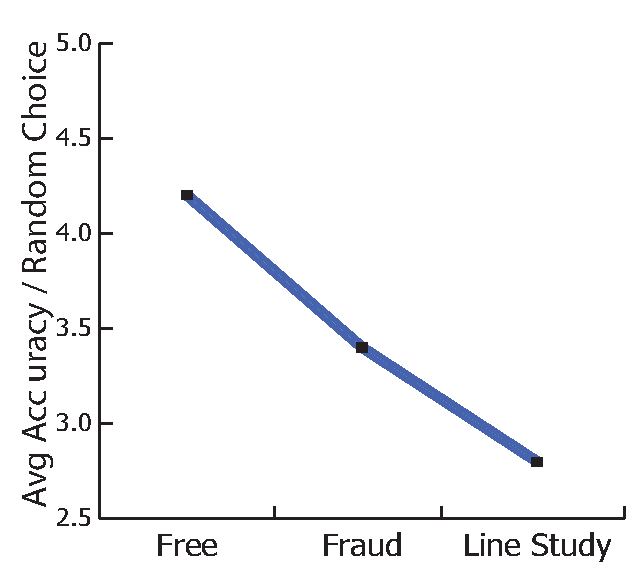
\includegraphics[width=0.42\textwidth]{images/sketchConstraints}
%  \caption{A plot of the ratio between SAR accuracy and random chance on all the datasets included in this paper. The datasets are organized on the horizontal axis in the order of increasing amount of sketch constraints. We see that the more constraints are added to how artists sketch, the less discriminative their strokes become.}
%  \label{crossDatasetsPlot}
%\end{figure}

%\vspace{-2mm}
\noindent\textbf{Fraud Recognition Experiment.} Here, we setup a fraud recognition experiment (original vs. fraudulent) that predicts SAR performance in a real-world scenario. It is unrealistic to assume that the SAR classifier will have access to fraudulent training examples from \emph{all} artists. However, we expect that when more fraudulent samples are used in training, SAR's test performance on fraudulent sketches from artists, who were \emph{not} included in training, will improve. In other words, knowing more about how fraud \emph{looks} like will help SAR better detect sketch fraud, even for fraudulent artists whose sketches are not trained on. To validate this expectation, we train the SAR binary (fraud vs. original) classifier with fraudulent sketches from increasingly more fraudulent artists (i.e. from 1 to 5 artists). In each case, 50\% of the original sketches are used for training (2-fold validation). Then, each SAR classifier is tested on the remaining original and fraudulent sketches. This means that SAR will always be tested on fraudulent sketches from artists, whose style has not been seen during training. In Figure \ref{fraudResults}, we plot the average test accuracy of SAR as the number of fraudulent artists used in training increases. Clearly, this result endorses our aforementioned expectation. In fact, SAR's fraud detection performance reaches 96\% when 5 of the 6 fraudulent artists are used for training and the $6^{\text{th}}$ for testing. Despite the extremely high similarity between fraudulent and original sketches, we conclude that SAR is able to effectively spot artistic fraud. Moreover, this result suggests that SAR can be used in an online active learning setup, where test samples are sequentially classified and in turn weighted and then used in re-training the classifier. %Our results show that SAR performance would tend to increase with more in this scenario.

%can be very useful in finding sketch fraud (e.g. from online sources), whereby its performance can improve when it adds

%This sheds light on SAR's applicability to the field of artistic fraud detection.

%\begin{figure}[ht]
%\centering
%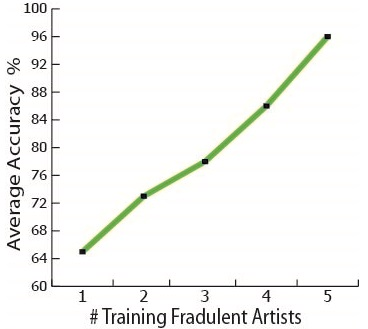
\includegraphics[width = 0.4\textwidth]{images/fraudResults}
%\caption {Fraud detection performance improves as more fraudulent artists are used in training even though testing is done entirely on sketches from fraudulent artists that are not included in training.}
%\label{fraudResults}
%\end{figure}

%SAR is able to estimate how \emph{close} artists-in-training are to a particular style.
%For fair comparison, we use the same number of classes across all datasets.
\vspace{-2mm}
\subsection{Algorithmic Details} \label{subsec:variations}
\vspace{-2mm}
Varying the details of the different computational modules of SAR (refer to Figire \ref{pipeline}), leads to a variant of SAR. In this section, we investigate many of these variations and provide algorithmic details to reproduce the SAR classifier.

%a number of algorithmic variations, which we experimented with during the development of SAR in order to build the best possible computational model. %We include the following experiments and results with the aim to help others in the community in conducting similar research. %We also assess assessment of some of the techniques used in SAR by comparing them against different techniques.

%\vspace{-2mm}
\noindent\textbf{Feature Contribution.} Stroke segments are represented by 4 biologically inspired features, as discussed in Section \ref{subsec: featureExtraction}. Here, we study the contribution of each feature to SAR's discriminative power. To do this, we employ a conventional forward feature selection method that greedily determines which features (along with their importance weights) should be incorporated into the SAR classifier. This is a data-driven process, so different training-test splits of the dataset can lead to different feature selections and weights. By training SAR (with 2-fold validation) multiple times on the free style dataset, we accumulate an average selection weight for each feature (refer to Figure \ref{FeatureTypeCont}). We see that eccentricity and local consistency are the most discriminative followed by inflection and symmetry with no one feature dominating.

%It is obvious that for a feature type to be considered, it must have contributed for better authorship classification accuracy. However, in this section we show the contribution of each feature type as reflected by the number of attributes selected from each feature type using our feature selection algorithm. As shown in , both Eccentricity and Local Consistency have almost the same number of significant attributes followed by Inflection and finally Symmetry. Overall, all feature types have significant attributes in them and the differences between the number of selected attributes between  different features is not large.
%\begin{figure}[ht]
%  \centering
%  \includegraphics[width=0.3\textwidth]{}
%  \caption{The contribution of each feature type}
%  \label{}
%\end{figure}

%\vspace{-3mm}
\noindent\textbf{Variations in Stroke Segmentation.} To justify our stroke segmentation method (refer to Section \ref{subsec: segmentation}, we compare it against two baseline methods: manual and random stroke segmentation.
For manual segmentation, we asked 10 artists to manually segment sketches into strokes as they see fit, while in the random case, breakpoints are selected uniformly at random within each extracted stroke. We set a minimum length for each stroke segment to prevent singularities. SAR accuracy (2-fold) using each of the three segmentation methods on the free style dataset is summarized in Figure~\ref{segAlg}. Clearly, our automated segmentation method outperforms the other two. Similar to the human recognition result in Section \ref{sec:humanexps}, SAR improvement over manual segmentation lends more evidence to the fact that human performance is suboptimal in fine-grained tasks, such as authorship recognition.

%We compared the performance of our segmentation technique against manual and random segmentation methods by running the classification model using the three techniques and check the classification accuracy obtained. For manual segmentation, we manually attempted to segment the strokes at singular and inflection points while in random segmentation we segmented the strokes such that each segment is of a certain number of pixels chosen randomly. Comparison results are shown in ~\ref{segAlg} and it proves that our segmentation technique results in better classification accuracy and thus it is better in detecting a particular artist's sketching style when compared with manual and random segmentation methods.

%\begin{figure}[ht]
%  \centering
%  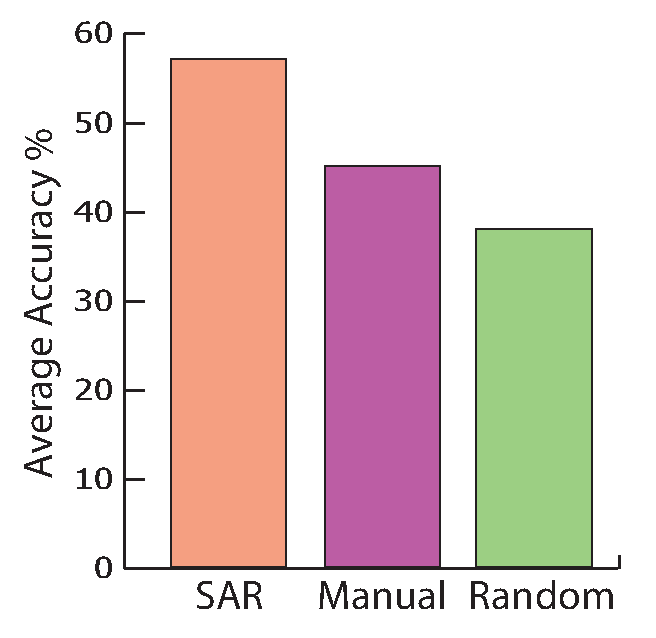
\includegraphics[width=0.3\textwidth]{images/segAlg}
%  \caption{SAR accuracy on the free drawing dataset when its segmentation method is replaced with a manual or random one. The inherent segmentation in SAR outperforms manual segmentation by around 15\% and random segmentation by around 20\%.}
%  \label{segAlg}
%\end{figure}

%\vspace{-3mm}
\noindent\textbf{Silhouettes vs. All Strokes.} In many cases (e.g. the Mickey Mouse cartoon character), the silhouette of a sketch can be very discriminative, so much so, that silhouettes have been used as primary features in other recognition tasks (e.g. action recognition \cite{li2008expandable}). Here, we study how discriminative silhouette stroke segments are on their own within the SAR pipeline. In Figure ~\ref{silAssesPlot}, we use two datasets to compare SAR accuracy when stroke segments are taken from the silhouette alone or from the entire sketch. Interestingly, silhouettes seem to be quite discriminative in their own right, as SAR performance remains high even when only silhouettes are used. In fact, including stroke segments from the sketch interior only improves accuracy by about 10\%.

%is only improved by about 13\% when internal stroke segments are added to silhouette stroke segments. This is a strong indication of the importance of silhouettes in determining sketch authorship.


%it is commonly understood that silhouettes \emph{alone} can contribute very rich information, so much so, that they have been used as primary features in other recognition tasks (e.g. action recognition \cite{silhaction}) \B{missing ref}. In fact, many objects and shapes (e.g. the Mickey Mouse cartoon character) can generally be recognized when just their silhouettes are shown.

%For the task of authorship recognition, we study how discriminative silhouette stroke segments are by themselves.  As shown Figure ~\ref{silAssesPlot}, SAR accuracy on the character dataset is only improved by about 13\% when internal stroke segments are added to silhouette stroke segments. This is a strong indication of the importance of silhouettes in determining sketch authorship.

%including the internal strokes to the silhouettes have just contributed around 10\% to the average classification accuracy and this gives a strong indication of the importance of silhouettes strokes in comparison with all the strokes when used to classify sketch authorship.

%The reason we gave the silhouettes this attention and follow that division is because they contribute a large portion of the entire sketch. Moreover, objects and shapes can generally be recognized when showing just their silhouettes. For example, a famous cartoon character like Mickey Mouse can be easily recognized from its silhouettes and one can recognize a sketch of an object like a table or a pen also by looking at their boundary. Thus, we assumed that silhouettes strokes can play a key factor in recognizing authorship among similar sketches as well.  As can be seen in ~\ref{silAssesPlot}, including the internal strokes to the silhouettes have just contributed around 10\% to the average classification accuracy and this gives a strong indication of the importance of silhouettes strokes in comparison with all the strokes when used to classify sketch authorship.

%\begin{figure}[ht]
%  \centering
%  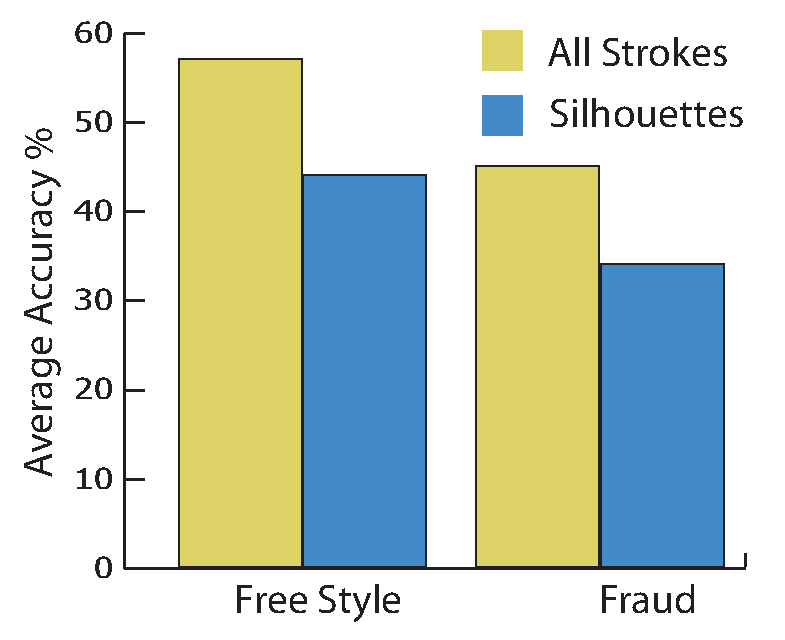
\includegraphics[width=0.3\textwidth]{images/sillVsInternal}
%  \caption{SAR accuracy on 3 sketch datasets where stroke segments come from either %silhouettes only or from the entire sketch. Adding internal stroke segments %\emph{does} improve accuracy but the improvement does not exceed 10\% across all %datasets.}
%  \label{silAssesPlot}
%\end{figure}


%\vspace{-3mm}
\noindent\textbf{Effects of Digitization.} As mentioned in Section \ref{subsec: segmentation}, stroke segments are extracted from a sketch using the well-known Adobe Live Trace digitization technique. The level of digitization is controlled by the user to tradeoff faithfulness to the original sketch with compactness of representation. For instance, high levels of digitization tend to smooth out strokes, thus, masking aspects of the artist's intrinsic style and possibly affecting SAR performance. To investigate the effect of digitization on SAR, it is applied to the fraud dataset after applying three distinct levels of digitization on its sketches. We report the average accuracies in Table \ref{table:digitization}. As expected, the higher the digitization level), the lower the SAR accuracy is. This result suggests another application that could benefit from SAR, namely the quantitative assessment of various digitization techniques. SAR can conceivably be used to evaluate how much of the unique sketching style is preserved after digitization.

%digitized sketches to the and evaluate them based on how the artistic style is preserved after digitization.

%In order to be able to extract all the strokes of a given sketch, we use Adobe Live Trace digitization technique which changes a bitmap image into vector. By tracing a sketch, a digitized version is created and Adobe users can control the level of detail and how the tracing is filled. One concern we had was; would the digitization had an influence on the artistic style such that recognition of a sketch authorship is disturbed? We asked this question after noticing that some of the artists' strokes details were smoothed out in the digitized version. With the aim to verify this, we ran SAR on three different sets of silhouettes strokes using the entire Fraud Experiment dataset discussed earlier. First, we applied SAR on the original silhouettes of the sketches. Next, we compared the obtained classification accuracy against 2 different types of the digitized silhouettes created using 2 digitization levels from the Adobe Live Trace options. The first level of digitization uses the best and the tightest approximation to the bitmap sketch while the second level uses the least tight approximation i.e. the resulted silhouettes are very smoothed out. The experiment results showed that the best classification accuracy is obtained by using the non-digitized sketches, then the tightly digitized sketches and finally the loosely digitized sketches as shown in ~\ref{table:digitization}. This indicates that digitization influences the artistic style and encourages the need of digitization techniques that can preserve the artist's unique strokes as best as possible. This also spots the light on one of the useful uses of SAR as it can be used to compare and assess different digitization techniques and evaluate them based on how the artistic style is preserved after digitization.

\vspace{-1mm}
\begin{table}[!htbp]
\caption {Effects of digitization on SAR accuracy. Sketches from the free style dataset are processed using three levels of digitization in Adobe Live Trace. SAR accuracy decreases significantly with higher levels of digitization.}
\label{table:digitization}
\vspace{-2mm}
\centering
\small
\begin{tabular}{c | c | c}
level of digitization& leave-one-out & 2-fold cross validation \\ \hline

%Original Sketch         & 48 &  45\\
Low       & \textbf{51} &  \textbf{45}\\
Medium       & 42 &  39\\
High      & 28 &  23\\
\end{tabular}\vspace{0mm}
\end{table}


%\vspace{-3mm}
\noindent\textbf{Style not Content.} SAR is designed to represent and classify artistic sketch style, while not being significantly sensitive to sketch content in general. This is a primary factor that distinguishes SAR from existing shape matching techniques discussed in Section \ref{subsec: shapematching}. In fact, our experiments show that sketches of different content (objects) drawn by the same artist tend to have more similar BoW features than sketches of the same content drawn by different artists. For instance, the BoW feature of a flower drawn by one artist is more similar to a butterfly drawn by that artist than the feature of the same flower drawn by another artist, as illustrated in Figure \ref{styleVsContent}. To quantify this observation, we use a normalized Gaussian similarity measure $s(\mathbf{I}_1,\mathbf{I}_2)$ based on the Euclidean distance between two BoW features. From the free style dataset, we randomly select a sketch $\mathbf{I}_i^A$ drawn by artist A and the same sketch $\mathbf{I}_i^B$  drawn by another artist B to compute $s(\mathbf{I}_i^A,\mathbf{I}_i^B)$. We then randomly select a sketch $\mathbf{I}_j^A$ drawn by A with $i\neq j$ and compute $s(\mathbf{I}_i^A,\mathbf{I}_j^A)$. By performing this operation across the whole dataset, we compute the average inter-artist similarity $s(\mathbf{I}_i^A,\mathbf{I}_i^B)=68\%$ and the average intra-artist similarity $s(\mathbf{I}_i^A,\mathbf{I}_j^A)=89\%$. This result shows that SAR can abstract an artist's style from different sketch content. We would like, however, to emphasize that strokes are not completely independent from the content. For example, SAR cannot recognize the authorship of sketches of a single square if an author's training data \emph{only} includes circles. Therefore, SAR inherently assumes that the training data contains non-trivial sketches with sufficient stroke diversity characterizing the overall style of any particular artist.



%we randomly select a sketch drawn by one artist and use the euclidean distance as the similarity metric i.e. less euclidean distance implies more similar histograms. We then picked the same sketch object drawn by 2 other randomly selected artists. Results have shown that a sketch drawn by Artist A is 89\% similar to sketches drawn by the same artist while only 75\% and 68\% similar to the same sketch object drawn by artists B and C.

%Using the free style dataset, we randomly picked a sketch drawn by one artist and use the euclidean distance as the similarity metric i.e. less euclidean distance implies more similar histograms. We then picked the same sketch object drawn by 2 other randomly selected artists. Results have shown that a sketch drawn by Artist A is 89\% similar to sketches drawn by the same artist while only 75\% and 68\% similar to the same sketch object drawn by artists B and C.

%In this section we emphasize that our proposed authorship technique (SAR) provides an artistic style discrimination with no dependency on the sketching content. This is one of the factors that distinguishes SAR from existing shape matching techniques as discussed earlier in Section \ref{subsec: shapematching}.

%We show that various sketches of different objects sketched by one artist tend to have more similar histograms when compared against other sketches of the same content but drawn by another artist. In other words, a flower drawn by one artist has a representing histogram that is more similar to a butterfly drawn by that artist than the histogram of the same flower object drawn by another artist. Using the free style dataset, we randomly picked a sketch drawn by one artist and use the euclidean distance as the similarity metric i.e. less euclidean distance implies more similar histograms. We then picked the same sketch object drawn by 2 other randomly selected artists. Results have shown that a sketch drawn by Artist A is 89\% similar to sketches drawn by the same artist while only 75\% and 68\% similar to the same sketch object drawn by artists B and C.

%as illustrated in Figure ~\ref{styleVsContent}.

\begin{figure}[ht]
  \centering
  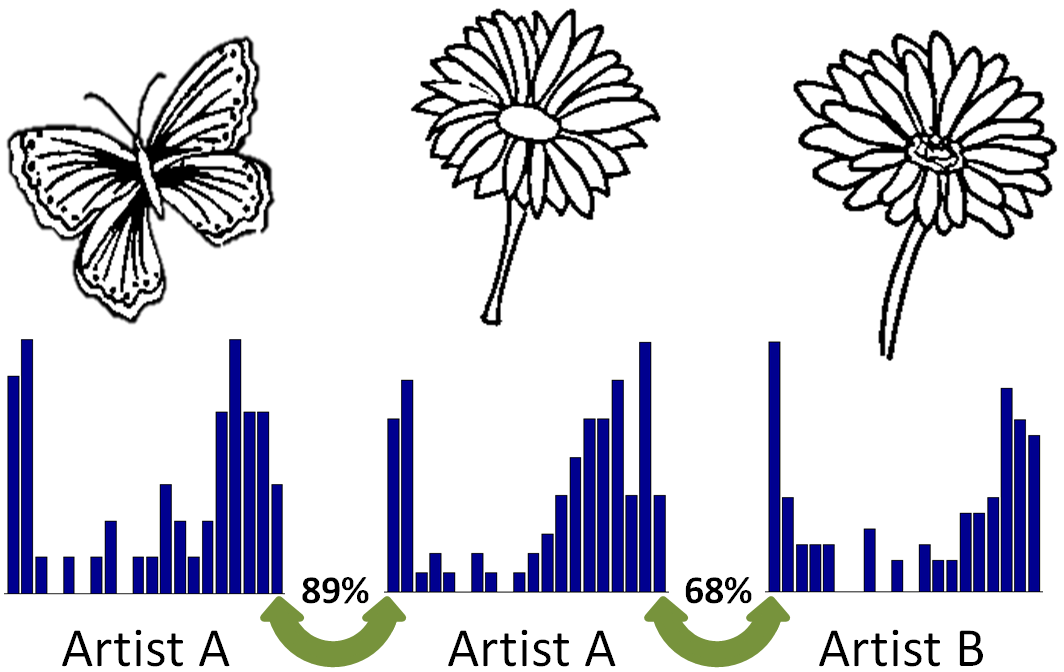
\includegraphics[width=0.5\textwidth]{images/styleVsContent2.png}
  \caption{A visual comparison between the BoW features of three sketches from the free-style dataset: a flower drawn by Artist A (middle), a butterfly drawn by Artist A (left), and the same flower object drawn by Artist B (right). From the features themselves and their average pairwise similarity scores, we see that SAR discrimination abstracts artistic style and is not significantly affected by sketch content.}\vspace{-2mm}
  \label{styleVsContent}
\end{figure}


\iffalse
\subsection{Human Vs. SAR.}
In this section, we summarize the difference in recognition performance between human subjects and our SAR automated system.

we compare human performance against our authorship recognition computational model. The first user study was built using the free style sketching dataset and our user study shows that people can successfully recognize the authorship of a sketch among 7 different artists with an average accuracy of 36\% and with a standard deviation of 10\%, using a sample of more than 2000 participants. SAR, on the hand, recorded an accuracy of 60\% and a standard deviation of 8\% when applied to the same dataset and using the same setup as in the user study. We also conducted another user study which involved 25 artists and using the fraud experiment datase. Artists were asked to distinguish fraudulent and original sketches using samples of both. User study results showed that given a set of sample sketches, artists can distinguish between fraudulent and original sketches with an average accuracy of 52\% and a standard deviation of 10\% while SAR classified fraudulent and original sketches under a setup similar to the user study with 96\% accuracy and with a standard deviation of 14\%. As can be seen, SAR outperformed human performance in classifying the authorship of similar sketches of which we conclude that SAR is predicted to be a useful tool to assist people and professionals in distinguishing authorship of sketches.
\fi


\vspace{-3mm}
\section{Applications} \label{sec:app}
\vspace{-2mm}
\begin{figure*}[htbp!]
\centering
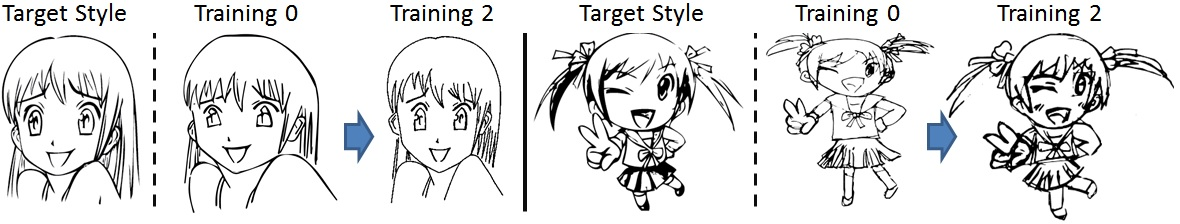
\includegraphics[width = 1.0\textwidth]{images/trainingSamples}
\vspace{-4mm}\caption {Samples sketches drawn by artists at the first and final stages of training along with the target style sketches. Sketches on the left correspond to the intermediate artist while ones on the right to the novice artist. The progress in their sketching styles is noticeable for both artists but more so for the novice one.}
\label{trainingSamples}\vspace{-4mm}
\end{figure*}

In this section, we show SAR's feasibility in two useful applications other than sketch fraud detection, namely sketch style training and sketch synthesis evaluation.

%various applications that require the comparison between artists' sketching styles (e.g. fraud detection and teaching artistic style).

\vspace{-2mm}
\subsection{SAR for Sketch Style Training}
\vspace{-2mm}
Knowing that an artist's sketching style is dynamic (i.e. it evolves over time), how persistent is it when artists undergo extensive training for the explicit purpose of altering their style and adopting another? For example, this type of training is administered in major cartoon companies (e.g. Walt Disney), usually for months on end. For this purpose, we develop a SAR-based application that allows artists, designers, and animators in-training to quantify their progress in adopting the \emph{target} style of a particular artist, whose sketches have been encoded in SAR. Trainees are able to draw and/or upload sketches to examine how close their artistic style has become to the target. We demonstrate this application next.

%%%%%%%%%%%%%%%%%%%%%
%% might want to re-add the fact that this same app can be used to show which artists have the same style and help them decide on which artists to work with.
%%%%%%%%%%%%%%%%%%%%%%


%For example, such an application can assist artists in deciding which artists to work with in group projects (based on high affinity values) or it can quantify how an artist-in-training is learning to draw with a particular sketching style. The later is what we are demonstrating next.

\noindent\textbf{Style Training Setup} We first determine a target style by finding a reasonably known artist, who has published his work online along with specific instructions on how to follow his drawing style. The target artist also provides YouTube videos showing how his sketches can be drawn step-by-step. We select fives sketches from his portfolio, specifically those with video instructions. Then, we identify three artists with varying levels of sketching and artistic experience (novice, intermediate, and advanced) to undergo the style training process. The advanced level artist is a professional with 10 years of experience and the intermediate artist has 3, while the novice artist only sketches as a hobby.

In the first stage of training, we ask all three artists to draw the five target sketches and then use the SAR-based tool to give them quantitative feedback on how similar their sketching style is to the target. The measure based on BoW features defined earlier in Section \ref{subsec:variations} is used to compute style similarity. In the second stage, we ask the artists to draw the sketches again after consulting a set of textual instructions on how to draw the target sketches. These instructions are obtained from the target artist's website. In the third stage, we provide the artists with their new SAR similarity scores along with instructional online videos. After submitting their newest sketches, we again compute their SAR similarity scores. Sample sketches of both novice and intermediate level artists at the first and last stages of training are shown in Figure \ref{trainingSamples}. It is obvious from these results that the novice artist has improved more significantly than the intermediate artist in adopting the target style.

%We first chose a set of 5 sketches drawn by one artist whose work is published over the internet with specific instructions on how to draw his sketches and how to follow his style. This is along with videos where the artist draws these set of sketches in step-by-step manner.

%After that, we trained SAR's application on these set of sketches. Next, we picked 3 artists such that each have a different sketching experience level. The first one is a novice artist with a minimum drawing experience while the second has an intermediate sketching level skills with only 3 years of practice and the third is an artist by profession with 10 years drawing experience.

%In the first stage of the training, we asked them to draw the chosen sketches and then use SAR to give them feedback on how their sketching style is close to the assigned sketches. In the second stage, we assigned them  the same sketches along with SAR's closure \% results and a set of instructions on how to draw the given sketches with that particular artistic style. We took those instructions from the website of that artist. In the third stage we provided them with a new SAR's closure \% results and videos on how to draw these specific sketches. Finally, we provided the participating artists with a SAR's closure \% which reflects how artists managed to modify their sketching style to match another artistic style. The training sketches used in this application at the 3 different will publicly be made available to allow for further testing and experimenting. Sample sketches of both novice and advanced level artists which visually shows how artists have evolved in their sketching styles is shown in Figure \ref{trainingSamples}.


\noindent\textbf{Style Training Results} Figure \ref{TrainingProgress} plots the evolution of the SAR similarity score throughout the 3-stage training process for each artist. As expected, each trainee's score increases with training. The novice artist exhibits an overall improvement of 10\%, which can be attributed to the explicit use of textual and video instruction for target training. The initial similarity scores for the intermediate and advanced level artists are much higher than the novice one, but they also exhibit an improvement of 4\% and 2\% respectively. The slight improvement by the advanced artist conveys how difficult it is for an artist with a well-defined style and extensive experience to adopt a new style, as well as, how much easier it is for a novice artist to do the same. Moreover, we expect that repeating these training stages (especially the last one) will further improve SAR similarity to the target style. Based on our results, we conclude that SAR can be successfully incorporated in the sketch training process (e.g. in major cartoon companies) to quantitatively monitor training progress. A training executable is available in the \textbf{supplementary material}. We will also release the training source code to extend this application to a larger set of sketches from more participating artists and to allow users to build their own training applications using their own sketch data.


%progress in approaching the style of the assigned set of sketches while intermediate level artist progressed by 4\%. Advanced artist, on the other hand, progressed with only 2\%. Closure results as proposed by SAR at the 3 different stages of the training is shown in Figure \ref{TrainingProgress}.

%This difference in progress \% between novice and advanced artists conveys how it is difficult for an artist with well defined style and long experience to draw with a new style while novice artists have higher ability to learn new styles. \SARA {In addition, advanced and intermediate artists have initially drawn the sketches in the first training stages with higher closure \% than novice artist.}




%The target sketches used in this application will be made publicly available to allow for further testing and experimentation.



%%%%%%%%%%%%%%%%%%%%%%%%%%%
%% add as future work: we want to develop a system that will suggest possible changes to the strokes in a sketch to become more like the target style
%%%%%%%%%%%%%%%%%%%%%%%%%%%

%Old Application: To this end, we present a straightforward application that demonstrates a training program that allows artists, designers, and animators to quantify their affinity to any given artist, whose sketches have been incorporated in training SAR. Users are able to draw or upload their sketches and examine how close their artistic style is to the pre-defined artists from  the different datasets included in this paper (refer to Section \ref{sec:datasets}). The executable of our application is available in the \noindent{\bf supplementary material}. For example, such an application can assist artists in deciding which artists to work with in group projects (based on high affinity values) or it can quantify how an artist-in-training is learning to draw with a particular sketching style as illustrated in \ref{training}. We aim to extend this application to a larger set of sketches from more participating artists and to allow users to build their own SAR classifiers on their own datasets by releasing the training source code.

%The answer to this question can be empirically verified by estimating SAR accuracy throughout the extent of the training period. We expect this accuracy

\vspace{-3mm}
\begin{figure}[ht]
\centering
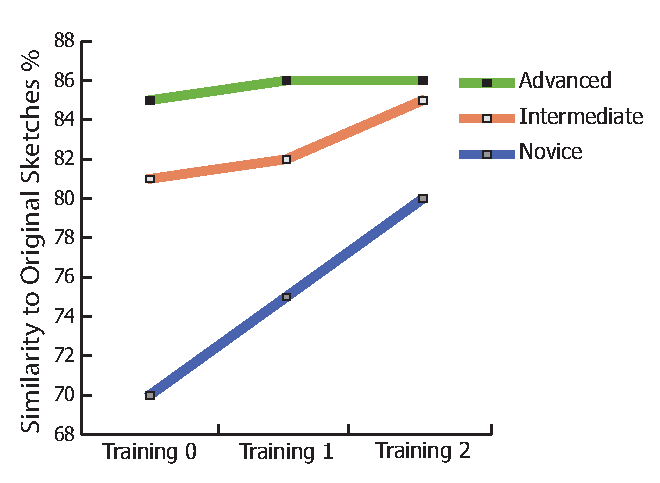
\includegraphics[width = 0.45\textwidth]{images/TrainingProgress}
\vspace{-2mm}\caption {SAR similarity-to-target scores for 3 novice, intermediate, and advanced level artists after 3 stages of training. The novice artist has the least score in the initial stage but progresses the most with training.}
\label{TrainingProgress} \vspace{-1mm}
\end{figure}


%\B{Change y-label to "Similarity to Target Style"}

\vspace{-2mm}
\subsection{SAR for Evaluating Sketch Synthesis Results}
\vspace{-2mm}
As mentioned in Section \ref{subsec: artisticanalysis}, there is a number of recent methods that focus on sketch synthesis and artistic style analysis. Their aim is to develop automatic sketch synthesis tools that mimic a particular artistic style. Most of these tools do not provide a quantitative assessment of how close the synthesized style is to the target one, thus, making it difficult to compare synthesis methods. A few of them however have validated their synthesis quality through extensive user studies, which are cumbersome to compile and require careful analysis. Since SAR is fully automatic, easy to use, and has proven style discrimination power (refer to Section \ref{subsec:recognition}), we propose to use it in quantitatively evaluating sketch synthesis methods without the need to conduct tedious user studies. To exemplify this application, we use SAR to analyze the synthesis results of Berger et. al. \shortcite{Berger:2013:SAP:2461912.2461964}. In their work, portrait sketches are synthesized from artistic styles of 7 artists, each of which drew 24 portrait sketches. The real and synthesized sketches are publicly available.


%A random choice classifier in this case has an average accuracy of 14\%.


We first use SAR to classify artistic style among the real portrait sketches only. In this case, SAR accuracy is 52\% (leave-one-out) and 50\% (2-fold), as compared to random chance accuracy of 14\%. When classifying only synthesized sketches, we obtain 54\% accuracy (leave-one out) and 51\% accuracy (2-fold) respectively. The  similarity in performance between the two scenarios suggests that the synthesized portraits are as hard to distinguish as the real ones and that the synthesis tool of \cite{Berger:2013:SAP:2461912.2461964} maintains a very similar amount of style diversity as in the real sketches. Next, we use SAR to classify the real sketches using the synthesized ones only as training and vice versa. In this case, SAR accuracy dropped to 26\% (leave-one-out) and 25\% (2-fold). This performance \emph{drop} can be used as a quantitative measure of synthesis quality, as it allows for comparison between different synthesis methods. In fact, an ideal synthesis tool should produce a SAR accuracy drop close to zero, since the style of the synthesized sketches should be undistinguishable from that of the real sketches.

Our results are on par with those of the three user (perceptual) studies conducted by Berger et. al. \shortcite{Berger:2013:SAP:2461912.2461964}. In fact, we setup the SAR classification experiments above to follow the same setup used in these user studies, where the only difference between the two is that SAR performs the classification automatically without any human feedback. The participants in the user studies registered a very similar accuracy when classifying the real and synthesized portraits separately (as did SAR). More importantly, the drop in classification by human participants is around 20\%, which is comparable to the 25\% drop reported by SAR. This result validates that SAR can be used to automatically and quantitatively evaluate sketch synthesis tools, without the need for user studies.


%To assess their synthesized results, they conduct 3 user studies involving 20 participants. In the first study, they asked participants to match a query real sketch to the artist they think drew it based on samples of real sketches of each artist. The second study, on the other hand, was the same but synthesized sketches were given in the query and in the provided samples. Participants registered similar accuracy in both studies which is aligned with our automated results shown above regardless of the fact that human performance was overall higher. In the third study, they asked participants to classify synthesized sketches to a collection of real sketches and vice versa. Participants performance dropped down by around 20\% compared to the first 2 studies which is the same amount of drop obtained by SAR. Their user studies provided us with a reliable baseline to assess SAR accuracy results.

%\textbf{Evaluation}
%Berrge et. al. \shortcite{Berger:2013:SAP:2461912.2461964} have conducted similar user studies to assess their synthesize results which involved a total of 20 adults and simulates a leave-one out cross validation scenario. Our automated results are aligned with their perceptual study results as follows: In classifying synthesize and real sketches separately, participants were 76.4\% and 72.4\% accurate respectively. SAR automated results, on the other hand was almost 20\% less but consistent with the user study results in terms of the minimum differences between classifying real and synthesized sketches.

%In another study, they asked participants to classify synthesized sketches to a collection
%of real sketches and vice versa. Participants performance dropped to 48\% and 50\%. Accuracy results of SAR went down by the same amount to become 25\%.

%This shows how challenging it is to build an accurate automatic replication of an artist's style as explained by the differences in the results above for both SAR and the user study they provided.

%. However, this was not the case in the portrait sketch dataset as the classification accuracy dropped down to 25\%.


%In this section we present an application that we built by utilizing the best performing computational model described in the previous sections. It makes use of all the different datasets provided in this work. Our application spots the light on one of the areas in which SAR can serve and that is analysis of artistic styles among different artists.

%We demonstrate a training program that allows artists, designers and animators to test their affinity to any given artist, whose works have been incorporated into the machine learning part of the program. Users are able to draw or upload their sketches and examine how close their artistic style to our defined artists who participated in creating the different datasets provided in this paper. Such application can for example assist artists to decide with which artists to work with in group projects or It can assess how an artist's style is approaching another style over training. We hope to see an extension of our application using a variety of artists sketches examples. The executable of our application is available in the \noindent{\bf supplementary material.}


\vspace{-3mm}
\section{Conclusions and Future Work}\label{sec:conclusions}
\vspace{-1mm}
In this paper, we shed light on a new direction in sketch analysis, namely authorship recognition through stroke analysis. We propose a stroke authorship recognition (SAR) approach that discriminates between artistic sketch styles based on the choice and frequency of use of basic strokes. From our extensive experiments and user studies, we provide empirical evidence regarding four interesting conclusions related to sketch analysis.

%In this paper, we propose a novel stroke authorship recognition (SAR) method that sheds light on a new direction in sketch analysis, namely authorship recognition through stroke analysis. To discriminate between authors based on their choice and frequency of use of strokes in their sketches, SAR focuses on representing each sketch image as a histogram of stroke segments from a learned universal dictionary. From our extensive experiments and user studies, we provide empirical evidence regarding four interesting conclusions related to sketch analysis.

%\begin{itemize}
%\item Based on results in Section \ref{subsec:recognition}, we conclude that SAR \emph{does} encode unique and consistent characteristics of an artist's sketching style, which are in turn used to discriminate one artist's sketches from others. A particular outcome of this result is SAR's ability to successfully detect fraudulent sketches given a set of original sketches. This conclusion justifies SAR's applicability to important real-world tasks, such as sketch fraud detection (e.g. for design patents and cartoon characters) and training/teaching artistic style.
%
%\item Interestingly, the extent to which SAR can be used for discrimination is highly dependent on the sketching constraints imposed on the artist. Although overall SAR accuracy decreases with more constraints, unique elements of artistic style are still preserved even under the strictest of constraints (fraud).
%
%\item We identified that a sketch's silhouette is a richer source of discriminative information than internal strokes in general. We validate the choice of our proposed segmentation method from a classification point-of-view, as well as, determine the optimal levels of digitization needed for accurate representation.
%
%\item All our conclusions are made possible by compiling multiple sketch datasets with various sketching constraints and content. Our extensive user studies empirically validate the difficulty of this fine-grained classification problem and indicate that our SAR approach can improve upon human performance. All the compiled data (datasets and user studies) will be made publicly available to enable further research on this exciting topic and to allow for quantitative comparison with future methods.
%\end{itemize}


\emph{Uniqueness of Sketch Style.} Based on results in Section \ref{subsec:recognition}, we conclude that SAR \emph{does} encode unique and consistent characteristics of an artist's sketching style, which are in turn used to discriminate one artist's sketches from others. This result validates SAR's applicability in important real-world tasks, such as sketch fraud detection (e.g. for design patents and cartoon characters) and training/teaching artistic style.

\emph{Style and Sketch Constraints.} The extent to which SAR can be used for discrimination is dependent on the sketching constraints imposed on the artist. Although overall SAR accuracy decreases with more constraints, unique elements of artistic style still persist even under the strictest of constraints (fraud).

\emph{Silhouettes.} We identify that a sketch's silhouette is a richer source of discriminative information than internal strokes in general. %We validate the choice of our proposed segmentation method from a classification point-of-view, as well as, determine the optimal levels of digitization needed for accurate representation.

\emph{Human Performance.} Our extensive user studies empirically validate the difficulty of this fine-grained recognition problem and indicate that SAR can improve upon human performance. All the compiled data (datasets and user studies) and source code will be made publicly available to enable further research on this exciting topic and to allow for quantitative comparison with future methods.


%However, since styles change dynamically with time, we believe that this uniqueness can

%The low-level image features we use to describe stroke segments, yet simple, are



%where sketches of different artists are analyzed with the aim to discriminate their authorship.
%
%It was initiated by first asking whether strokes are unique to the artist who draws them and then extended to experiment how such uniqueness can classify an authorship of a sketch. In our method, we extract inherent characteristics on boundary and internal curve strokes and use them to represent each sketch as a histogram of universal stroke segments. To show the discriminative power of SAR, we conducted extensive classification experiments on several datasets, which we form using sketches of collaborating artists. Experimental classification results across all datasets were much higher than random choice. This ,in turn, validates the effectiveness of SAR and proved that artists exhibit uniqueness and consistency in their sketches. Moreover, SAR showed competency in detecting fraudulent sketches with 95\% accuracy when tested on the fraud dataset compiled in this work. To reflect on the challenge of recognition involved, we conducted a couple of user studies designed using the same learning circumstances available for training SAR and used them to compare human performance with the computational results of SAR. Results showed that SAR outperformed human abilities in sketch authorship recognition.
%
%We have also experimented SAR on different techniques with the aim to come up with the best computational model with the highest classification accuracy among different datasets. We share our experimental results of a number of algorithmic variations involved in the development of SAR. First, We have tested our proposed segmentation algorithm against random and manual segmentation methods to validate its effectiveness. Moreover, we found that the silhouettes of a sketch convey lots of information regarding authorship of a sketch when compared to all the strokes. Finally, we experimentally proved how using digitization techniques for strokes extraction can affect the originality of the sketch.


%\noindent{\bf Limitations and future directions.  }
%
%- Internal stroke extraction takes place in a pre-processing step.
%
%- we need digitization techniques that do not cause any changes in the artistic style
%
%- Need of large scale datasets across multiple artists over time and using same artists, different constraints, add training
%
%- Add more local features that can reflect new aspects of artist's style
%
%- combine local features with global shape information (will this give more information!)
%
%- We are interested in applying SAR to 3D curves and shapes in the future
%
%- Design useful applications (list examples) such as artistic fraud detection, design patents and brand marking
%\vspace{-3mm}
\textbf{Future Work} We aim to improve the discriminative nature of SAR by improving the quality of the learned universal stroke segment dictionary. One way to do this is to investigate how strokes are actually generated by the artists. This can be done by tracking their hand movements and how they hold the pencil/pen while sketching. We believe this will provide us with more information about an artist's style of sketching. Although the segmentation process is currently viewed as a pre-processing step in SAR, we aim to investigate how supervised information (artist labels) can be incorporated in this process (possibly through supervised dictionary learning) in order to produce stroke segments that are inherently discriminative. Furthermore, we will extend our compiled datasets to more sketches and contributing artists.


%We have presented a new method of shape representation and authorship classification. It is based on analyzing local features of the sketch's silhouettes and internal strokes which are then used to represent a sketch as a histogram of universal strokes segments. The later representation is used in a k-NN based authorship classification model. The proposed method is applicable to sketches in various sizes, and invariant to non-rigid motion, scaling and rotation. Experimental results on a number of datasets we compile in this work demonstrate that our method has a good performance on authorship discrimination and classification.




%Towards the end of this paper we demonstrate a couple of applications which are built using the best performing computational model. The first one is an artistic fraud detection application that is based on one of the datasets we are providing. The second application is a training program that allows artists, designers and animators to test their affinity to any given artist, whose works have been incorporated into the machine learning part of the program, it is also designed based on one of our datasets.


\bibliographystyle{eg-alpha}
%\bibliographystyle{eg-alpha-doi}
\bibliography{egbibsample}
\end{document}
